%
%% Please do not remove author note!
%%%
%%%% Created by Kacper B Sokol (k.sokol.2011 [at] my.bristol.ac.uk)
%%%
%% Please do not remove author note!
%

\documentclass[11pt, letterpaper]{article}            % report | leqno, pdflatex

% \usepackage[]{algorithm2e}
% \usepackage[usenames,dvipsnames]{color}
% \usepackage[letterspace=3pt]{microtype} % linespacing

\usepackage[left=3.17cm, right=3.17cm, bottom=2.54cm, top=2.54cm]{geometry}
\usepackage{graphicx}                                                 % graphics
\usepackage{color}                                              % custom colours
\usepackage{lipsum}                                        % just a space filler
\usepackage{soul}                                               % letter spacing
\definecolor{natc}    {RGB}{021,055,090}
\definecolor{subc}    {RGB}{121,121,121}
\definecolor{headc}   {RGB}{034,065,094}
\definecolor{headerc} {RGB}{127,145,173}
\definecolor{footerc} {RGB}{128,128,128}
\definecolor{footerc1}{RGB}{192,192,192}
\definecolor{linec}   {RGB}{237,237,237}
\usepackage[absolute]{textpos}      % absolute positioning of images | showboxes
\usepackage{cite}                                                        % BiTeX
\usepackage[square]{natbib}                                   % Harvard citation

\usepackage{datetime}                                              % custom date
\newdateformat{motd}{\monthname[\THEMONTH] \THEYEAR}               % custom date

\usepackage{fontspec}                                      % all different fonts
\usepackage{xcolor}
\usepackage{titlesec}
\defaultfontfeatures{Ligatures=TeX}
\setsansfont{Arial}
\setmainfont{Times New Roman}
\titleformat*{\section}{\fontsize{16}{18}\color{headc}\bfseries\sffamily}
\titleformat*{\subsection}{\fontsize{13}{15}\color{headc}\bfseries\sffamily}
\titleformat*{\subsubsection}{\fontsize{11}{13}\color{headc}\bfseries\sffamily}
\newfontfamily\headerfont[Ligatures=TeX]{Calibri}
\newfontfamily\footerfont[Ligatures=TeX]{Times New Roman}


\usepackage[linktocpage=true]{hyperref}                         % click-able ToC
\usepackage{tocloft}
\renewcommand{\contentsname}                               % ...
    {\fontsize{16}{18}\color{headc}\bfseries\sffamily      % ...
    Table of Contents}                                     % change name for ToC

\setcounter{tocdepth}{3}
\cftsetindents{section}{0.0em}{1.0em}
\cftsetindents{subsection}{1.0em}{2.0em}
\cftsetindents{subsubsection}{2.0em}{3.0em}
% \cftsetindents{paragraph}{0.5in}{0.5in}
% \makeatletter \renewcommand*\l@section{\@dottedtocline{1}{1.5em}{2.3em}} \makeatother
\makeatletter \renewcommand*\l@section{\@dottedtocline{0}{0.0em}{1.5em}} \makeatother
% \renewcommand{\cftsecfont}{\fontsize{19}{13}\color{headc}\bfseries\sffamily}


% define headers and footers
\usepackage{etoolbox,fancyhdr,xcolor}
\pagestyle{fancy}
\newcommand{\footrulecolor}[1]{\patchcmd{\footrule}{\hrule}{\color{#1}\hrule}{}{}} % footer colour
\fancyhead{} % clear all header fields
\renewcommand{\headrulewidth}{0pt} % no line in header area
\fancyhead[LE,LO]{\headerfont\fontsize{9}{11}\selectfont\color{headerc}\textbf{CERN openlab Summer Student Report}}
\fancyhead[RE,RO]{\headerfont\fontsize{9}{11}\selectfont\color{headerc}\textbf{\the\year}}
\fancyfoot{} % clear all footer fields

%%%%%%%%%%%%%%%%%%%%%%%%%%%%%%%%%%%%%%%%%%%%%%%%%%%%%%%%%%%%%%%%%%%%%%%%%%%%%%%%
%%%%%%%%%%%%%%%%%%%%%%%%%%%%%%%%%%%%%%%%%%%%%%%%%%%%%%%%%%%%%%%%%%%%%%%%%%%%%%%%
%%%%%%%%%%%%%%%%%%%%%%%%%%%%%%%%%%%%%%%%%%%%%%%%%%%%%%%%%%%%%%%%%%%%%%%%%%%%%%%%
%%%%%%%%%%%%%%%%%%%%%%%%%%%%%%%%%%%%%%%%%%%%%%%%%%%%%%%%%%%%%%%%%%%%%%%%%%%%%%%%
%%%%%%%%%%%%%%%%%%%%%%%%%%%%%%%%%%%%%%%%%%%%%%%%%%%%%%%%%%%%%%%%%%%%%%%%%%%%%%%%
%%%%%%%%%%%%%%%%%%%%%%%%%%%%%%%%%%%%%%%%%%%%%%%%%%%%%%%%%%%%%%%%%%%%%%%%%%%%%%%%
\usepackage[]{algorithm2e}
\usepackage{listings}
\definecolor{navyb}{RGB}{100,043,054}
\definecolor{darkgreen}{RGB}{070,155,070}

\newcommand\mycommfont[1]{\footnotesize\ttfamily\textcolor{blue}{#1}}
\newcommand{\ts}{\textsuperscript}

\usepackage{caption}
\usepackage{subcaption}

\usepackage{amsmath}
\usepackage{amsfonts}    % fancy maths font
\usepackage{mathrsfs}    % fancy maths font
\usepackage{dsfont}      % indocator finction
\usepackage{mathtools}
%%%%%%%%%%%%%%%%%%%%%%%%%%%%%%%%%%%%%%%%%%%%%%%%%%%%%%%%%%%%%%%%%%%%%%%%%%%%%%%%

\begin{document}

\begin{textblock*}{0mm}(-12.2mm,-0.3mm)\noindent \includegraphics*{./gfx/bg.png}\end{textblock*}
\begin{textblock*}{0mm}(144.3mm,238.3mm)\noindent \includegraphics*{./gfx/openlab.png}\end{textblock*}
\begin{textblock*}{150mm}(114.2mm,140.0mm)\noindent
\parbox{8cm}{\bfseries\sffamily\textbf{\fontsize{20}{20}\selectfont\color{natc}Making sense of data streams:}}\\[.3em]
\parbox{8cm}{\bfseries\sffamily\textbf{\fontsize{20}{20}\selectfont\color{natc}Complex Event Processing for Controls Applications}}\\[36pt]
{\bfseries\sffamily\textbf{\fontsize{16}{20}\selectfont\color{natc}\motd August 2014}}\\[18pt]
{\sffamily\fontsize{14}{20}\selectfont\color{subc}Author:}\\
{\sffamily\fontsize{14}{20}\selectfont\color{subc}Kacper B.\ Sokol}\\[18pt]
{\sffamily\fontsize{14}{20}\selectfont\color{subc}Supervisor(s):}\\
{\sffamily\fontsize{14}{20}\selectfont\color{subc}Filippo Tilaro}\\
{\sffamily\fontsize{14}{20}\selectfont\color{subc}Axel Voitier}\\[18pt]
\textbf{\bfseries\sffamily\fontsize{11}{20}\selectfont\color{subc}CERN openlab Summer Student Report 2014}

\end{textblock*}
~
\thispagestyle{empty}\newpage

\section*{Project Specification}
CERN is currently investigating the usage of data analysis technologies to study the behaviour of the industrial control systems. An activity related to these analysis is using \emph{Complex Event Processing} (CEP) tools to classify a real abnormal behaviour from one generated by a human intervention on the system.\\
In this study the Complex Event Processing classification is run over signals produced by variety of sensors and simulators. The selected tools is \texttt{Esper}. Presented here work consists of installing chosen tool, and developing the classification system with it to address given above merit.
\newpage

\section*{Abstract}
This project aims at building a tool to process live streams of data produced by various sensors and artificial generators. To this end, a \texttt{Java} code is written, which uses \texttt{Esper} \emph{Complex Event Processing} package to: receive data feeds, apply user defined rules and filters, and pass the resulting information to a clustering framework.\\
The last step employs \emph{Affinity Propagation} based clustering algorithm, which choice is motivated by its dynamic adaptation to number of clusters in the data. This is key feature in data streaming scenario as the number of clusters can evolve with time. Furthermore,~\citep{zhang2013data} have documented overall good performance of Affinity Propagation in cases of live data analysis.\\
Finally, presented here approach is compared and contrasted against static clustering algorithms applied to data gathered from streams incoming over one run of the program, followed by in-depth results analysis.\\[1cm]
\textbf{Keywords:} Esper, Complex Event Processing, Affinity Propagation, data streams
\let\thefootnote\relax\footnote{\noindent This report was written in \LaTeX.}\\
\newpage

{\fontsize{11}{13}\sffamily\linespread{1.750}\selectfont\tableofcontents}
\thispagestyle{fancy}\newpage

% Start footer here
\fancyfoot{} % clear all footer fields
\renewcommand{\footrulewidth}{0.4pt} % no line in header area
\footrulecolor{linec}
\fancyfoot[LE,LO]{\footerfont\fontsize{9}{11}\selectfont \textcolor{footerc}{\textbf{\thepage~$|$}}~\textcolor{footerc1}{\footerfont\so{\texttt{Page}}}} % \fontfamily{ppl}\selectfont

\section{Introduction}
Physicists at CERN are mainly concerned with event reconstruction. This implies collecting data first and then processing them. It is not possible with sensors data like pressure, or temperature. In case of abnormal behaviour, e.g.\ overheating, the action need to be taken instantly.\\
This study presents an approach to handle live data streams and analyse them ``on the fly'' to differentiate between noisy feed and real threats, hence produce human readable data inferences.\\

In machine learning, unsupervised clustering aims at discovering cluster structure underpinning the data (\citep{Flach:2012:MLA:2490546} extensively describes main concepts of machine learning). There are many state-of-the-art algorithms designed to solve this problem, nevertheless, majority of them deals with static data, forcing user to define many parameters prior to classification. The example of these might be a predefined number of clusters. Also, many of these algorithms need data with static distribution, and what is more static dataset, i.e.\ not changing with time.\\
The major study addressing these issues is presented by~\citep{zhang2013data}, who proposed clustering algorithm based on affinity propagation scheme that solves all of the above concerns: it adapts to patterns evolving in data by tracking current number of clusters, therefore it handles non-stationary data distribution; furthermore it can be easily adjusted to data streams.\\

I aim at extending presented by~\citep{zhang2013data} approach with \texttt{Esper} framework (\texttt{Esper} engine is briefly introduced by~\citep{Marinescu2006}). My concept facilitate modular feature extraction: user can change signal characteristics of interest while application is running; and it gives all advantages of time windowing provided by \texttt{Esper}.\\
I construct feature extraction system based on \texttt{EPL} statements and clustering solution capable of handling live data stream.\\

%The \texttt{EPL} language are simple human readable sentences defining features to be extracted using predefined handlers like average and standard deviation as well as functions written in Java.

\subsection{What is \emph{Complex Event Processing}}
\emph{Complex Event Processing} (CEP) is a software family facilitating complex analysis of high throughput live data feeds.\\
The concept behind it is similar to database queries, but instead of interacting with static data pool the extraction is done on live streams. It gives possibility of applying filters, functions, and statistical analysis to chosen part of signal by \emph{querying} it. \citep{Etzion:2010:EPA:1894960} presents comprehensive introduction to the topic.

\subsection{What is \texttt{Esper}}
\texttt{Esper} is a flagship software of Complex Event Processing tools family. It is capable of handling and analysing multiple independent incoming data streams. The main goal of analysis is to trigger user defined actions, e.g.\ if the temperature feed is above some level for given amount of time an additional cooling system can be deployed.\\

\texttt{Esper}'s main advantage is \emph{time windowing}, which allows to focus on a specific time period. The windowing can be done in multiple modes:
\begin{description}
    \item[Time] incoming data from last $t$ milliseconds/seconds/minutes/etc.\ are processed---sliding window.
    \item[Time batch] data are processed in $t$ milliseconds/seconds/minutes/etc.\ batches i.e.\ algorithm collects data for $t$ units of time, then process them, and repeats this cycle---fixed length interval windows e.g.\ $\left\{ [0, t); [t, 2t); [2t, 3t), ...\right\}$ where $0$ point is the start of our analysis.
    \item[Length] $n$ most recent events are processed---the order of arrivals is the only quantity of interest.
\end{description}

Moreover, \texttt{Esper} is capable of joining multiple, independent, asynchronous (events form one stream can be lively processed regardless of others) incoming signals for processing purposes. With proprietary \texttt{EPL} querying language the analysis is as simple as writing number of human readable statements.\\
One approach is to hard-code the EPL queries in the application but it is more convenient to provide them as a module (external plain text file) what gives flexibility of changing the queries without stopping the application.\\

Finally, \texttt{Esper} is available as a \texttt{Java} and \texttt{.NET} framework hence it is multi-platform and easy to incorporate into any application. It can work as both: local and server programme, where later solution facilitates on-the-fly changes like rules injection via AIP.\\

\subsection{Why to use it}
The major advantage of \texttt{Esper} is ability to process millions of events per second with low computational complexity and no time consuming read/write disk operations.\\
The data processing is describe by developers as ``\textbf{4-D}'' concept:
\begin{description}
\item[\textit{D}etect] events of interest.
\item [\textit{D}erive] events complying with specified rules.
\item [\textit{D}ecide] what to do based on gathered evidences---data.
\item [\textit{D}o] the action bonded with occurring event.
\end{description}

\subsubsection{Complex Event Processing at CERN}
I adopt the ``\textbf{4-D}'' flow to my application as follows:
\begin{itemize}
\item \emph{detect} incoming signals from the sensors (generators);
\item \emph{derive} the specified features from the signal;
\item \emph{decide} to send the features to clustering algorithm; and
\item \emph{do} the classification.
\end{itemize}

\subsection{Applications}
\texttt{Esper} is mainly used in high throughput data analysis services, where processing must be flexible and adaptable to constantly changing environment. The following examples show different aspects of \emph{Complex Event Processing}.

\subsubsection{Nuclear Power Plant}
While managing nuclear power station there are plenty of components whose malfunctioning may lead to a disaster, for example:
\begin{itemize}
\item to high core temperature,
\item failure of cooling pumps, or
\item abnormal seismic movements.
% \item weather forecast,
% \item electricity usage projections.
\end{itemize}
Only specific combination of these factors states should raise an alarm. For instance low flow of cooling liquid and constantly raising core temperature.\\
\texttt{Esper} is a great fit for this scenario. It allows to view the sensors readings in different time windows hence discover long and short term patterns. For instance, if the temperature raises slowly the trend will not be visible in last hour frame, but it will appear in week or month window. Discovering this long term property may prevent a disaster.

\subsubsection{Stock market exchange}
In this example we consider signals as all the real time price processes injected to \texttt{Esper}. We begin by filtering them with EPL statements to retrieve stocks of interest. Then, we use our financial knowledge to create inferences between them and perform complex analysis of price processes. We can also use weather forecast and news feed to gather some background. Combining all these rules can trigger market actions like: shares quantity, and buy/sell order; therefore increasing bidding speed and automatizing trading. Other approach could be to extract market statistics which can be used by financial advisers.


\section{Model of processing}
In this section I describe a model of processing used in the application, and presented in \textit{Figure~\ref{fig:model}}.\\

We divide the model into two main branches: \emph{off-line resources} and \emph{live data processing}.\\
The first one consists of
\begin{itemize}
\item \texttt{EPL} file (see \textit{Listing~\ref{lst:EPL}}), that defines the features to be extracted form the incoming signal (rules);
\item \texttt{CSV} file which serves as a data repository---signals are saved here for future analysis; and finally
\item data reconstruction script written in \texttt{Python}: \texttt{visualize.py}, which uses \texttt{CSV} data repository to plot signal and all extracted features against time as well as features against each other.
\end{itemize}
\emph{Live data processing} module consists of the following components:
\begin{description}
    \item[Signals layer] includes signal generators and signal feeds interfaces.
    \item[\texttt{Esper} layer] collects signals, and applies to them rules taken form \texttt{EPL} file. It also saves signals, extracted features, and time stamps to \texttt{CSV} repository. Finally, it performs defined actions, in this particular application it supplies them to clustering algorithm.
    \item[Events layer] transfers data (events) to clustering module.
    \item[Affinity Propagation Clustering layer] receives events and performs clustering on live data stream. Once a datum point is assigned to cluster, this information is appended to \texttt{CSV} repository.
\end{description}

\begin{figure}[htbp]
    \centering
    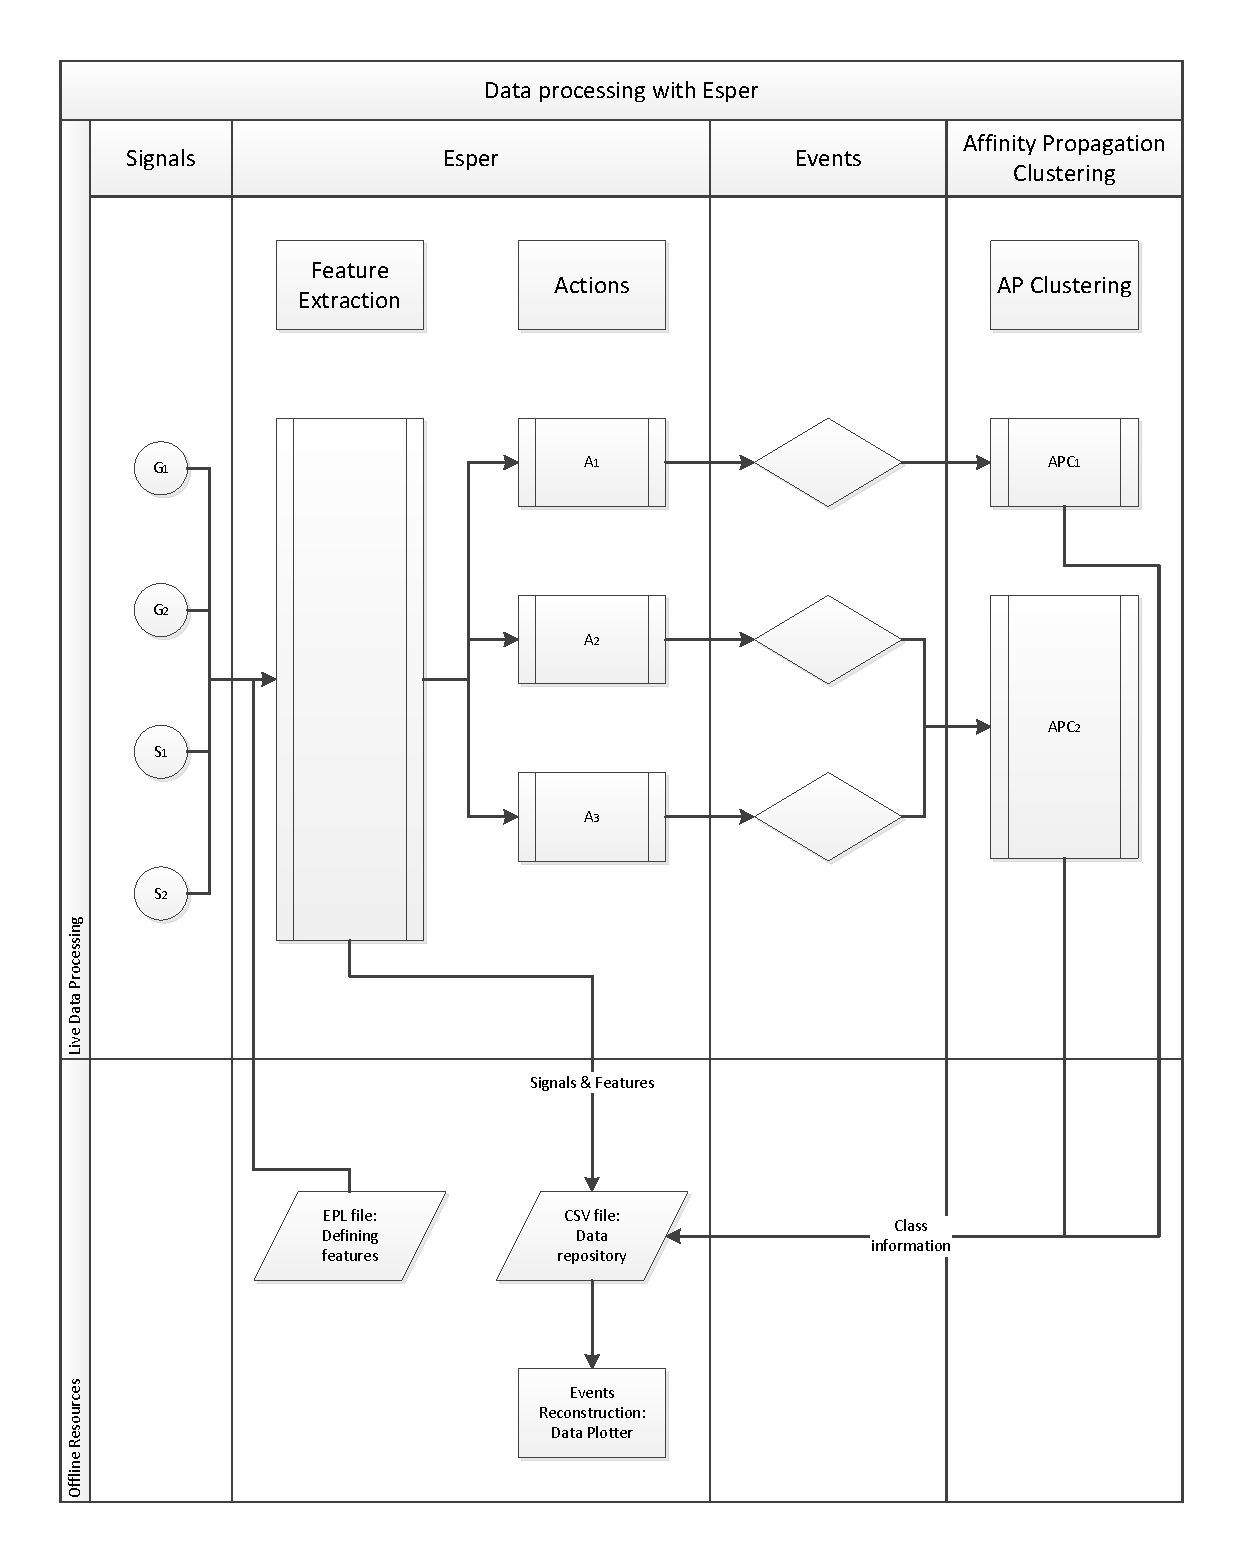
\includegraphics[width=\textwidth]{./gfx/model.pdf}
  \caption{Data processing model.\label{fig:model}}
\end{figure}

\subsection{Feeds and generators\label{sec:generators}}
A number of signal generators is implemented to test the framework:
\begin{itemize}
    \item \emph{sine} wave with normally distributed noise,
    \item \emph{cosine} wave with normally distributed noise,
    \item \emph{normal} distribution generator,
    \item \emph{uniform} distribution generator,
    \item \emph{multivariate normal} distribution generator.
\end{itemize}
The time between generated samples is modelled according to \emph{Poisson} distribution---it simulates pseudo-random signal occurrence.\\

The package also contains module which collects temperature readings from the electronic thermometer placed at CERN Prévessin site, and Yahoo! weather forecast feed for the same location. Both of them can be used as signal providers for the application.\\

In \emph{Esper} the easiest (and the one that I use) way to represent a signal is \emph{POJO}---Plain Old Java Object. Such object contains some properties---constants---like \texttt{currentValue} and \texttt{timeStamp}. Every event arriving from source is or can be converted to a POJO. Such container holding signal properties is delivered to the processing unit of \texttt{Esper} via \emph{listeners}.

\subsection{\texttt{Esper} engine}
The \texttt{Esper} engine runs in the background gathering signals from all indicated by user (see §\ref{sec:rules}) sources. It filters all these incoming data with \texttt{EPL} rules and delivers desired ones to corresponding listener (see §\ref{sec:listeners}).\\
The \texttt{Esper} framework is capable of running multiple servers simultaneously. It also allows to make changes to model of processing without stopping the server via provided API. This feature significantly increases usability of \texttt{Esper} as it prevents any data lose and allows fine-tuning.\\

\subsection{Rules: feature extraction\label{sec:rules}}
In presented model \emph{rules} decide what measures of data feed the user is interested in. They allow to get the value of the signal and apply built-in or \textbf{user-defined} filters on-the-fly.\\
\texttt{Esper} allows to either \emph{hard-code} the rules in a source code of a program, or read them in from external \texttt{EPL} file, alternatively they can be sent to the engine via API.\\
The \texttt{EPL} language is similar to database queries, but instead of fixed pool it uses part of stream selected by time-window.\\
%  which can be either specified in the code or deployed while engine is running

In my application I use rules as \emph{signal feature extractors}. In particular I am interested in:
\begin{description}
  \item[mean] signal average in given time period $\bar{v}$,
  \item[standard deviation] standard deviation in given time period $v_\sigma$,
  \item[$k$-lag] a difference between current value of the signal and n\ts{th} previous value i.e.\ $v_t - v_{t-n}$,
  \item[threshold] a user-defined function which thresholds the signal based on a single value $\mathscr{V}$,
  \item[current value] a current value of the signal $v_t$,
  \item[\texttt{FN}] a number of defined features,
  \item[\texttt{TS}] an assigns time-stamp $t$ of received signal.
\end{description}

The example of rules extracting above features are placed in \texttt{EPL} file shown in \emph{Listing}~\ref{lst:EPL}.\\
The \texttt{EPL} file consists of (in preserved order):
\begin{itemize}
  \item module name,
  \item dependencies that need to be imported,
  \item alias definitions i.e.\ short names for signals,
  \item rule name,
  \item rule description,
  \item rule body.
\end{itemize}
Generic rule starts with a \texttt{select} keyword. Then, features are extracted by applying functions to current signal value. For simplicity, each extracted feature is assigned an alias with \texttt{as} keyword. To clarify, in example given below variables \texttt{current} and \texttt{timer} are members of \texttt{randomGenerators.Sine} class---they are signal properties. Finally, \texttt{from} keyword is used to indicate which signal is used and \texttt{win:time(60 sec)} is placed to indicate time window of interest.\\
For convenience each file can contain multiple rules.

\vspace{1em}
\lstset{
  captionpos=b,
  frame=single,
    emph={module, import, create, schema, as, @Name, @Description, select, from, win:time},
    emphstyle={\color{navyb}\bfseries},
    caption=EPL file example.,
    label=lst:EPL
}
\begin{lstlisting}
module
  SpringfieldNuclearPowerPlant.engine.ExternalFeatureExtractor;

import
  featureExtractors.FeatureExtractor;

create schema SinTick  as randomGenerators.Sine;

@Name('Basic---Statistics')
@Description('Extract basic signal statistics to features')
select
avg(current) as F1,
stddev(current) as F2,
featureExtractors.FeatureExtractor.posNeg
  ( (current - prev(1, current)) ) as F3,
featureExtractors.FeatureExtractor.posNeg
  ( (current - prev(2, current)) ) as F4,
current as F5,
featureExtractors.FeatureExtractor.threshold
  (current) as F6,
6 as FN,
timer as TS
from SinTick.win:time(60 sec);
\end{lstlisting}


\subsection{Listeners for change\label{sec:listeners}}
A listener is a thread running in the background and acting upon arrival of new event---signal tick---according to some attached rule.\\
\texttt{Esper} gives user a flexibility to define multiple rules and listeners, and pair them in non-restrictive manner e.g.\ :
\begin{itemize}
\item multiple listeners are attached to a single rule,
\item one listener is attached to multiple rules,
\item one listener is bonded with one rule.
\end{itemize}

\noindent I use this module to pass features extracted from signals to clustering framework (see §\ref{sec:sclustering} for reference).

\subsection{Clustering with Affinity Propagation\label{sec:sclustering}}

\subsubsection{Live stream adaptation of clustering algorithms\label{sec:livestream}}
\citep{zhang2013data} presented a general framework for adapting an unsupervised clustering algorithm to data streams. Their approach can be used with any clustering algorithm that does not need a fixed, predefined number of clusters as a model parameter. This restriction motivates their use of \emph{Affinity Propagation} unsupervised clustering which is presented in more details in \emph{§}\ref{sec:AfinProp}.\\

The overview of their approach is presented in \emph{Figure}~\ref{fig:APC}.\\

The process begins by feeding the framework with stream of extracted features. The algorithm uses initial batch of data (user defined, fixed number of initialization points) to create first model.\\
Once the model is initialized, all incoming points are tested for fitting the model: if they do, they are appended to current model, and if they do not they are stored in \emph{reservoir}. Fitness test checks whether given point is an outlier with regard to current model.\\
There are two possibles events that can trigger model rebuild: full reservoir---its fixed size is defined by user, or positive outcome of \emph{change point detection} test on incoming stream---it detects ``significant'' and ``sudden'' change on the input stream. If any of these triggers fire, the model is rebuilt with data from reservoir.\\

\begin{figure}[htbp]
    \centering
    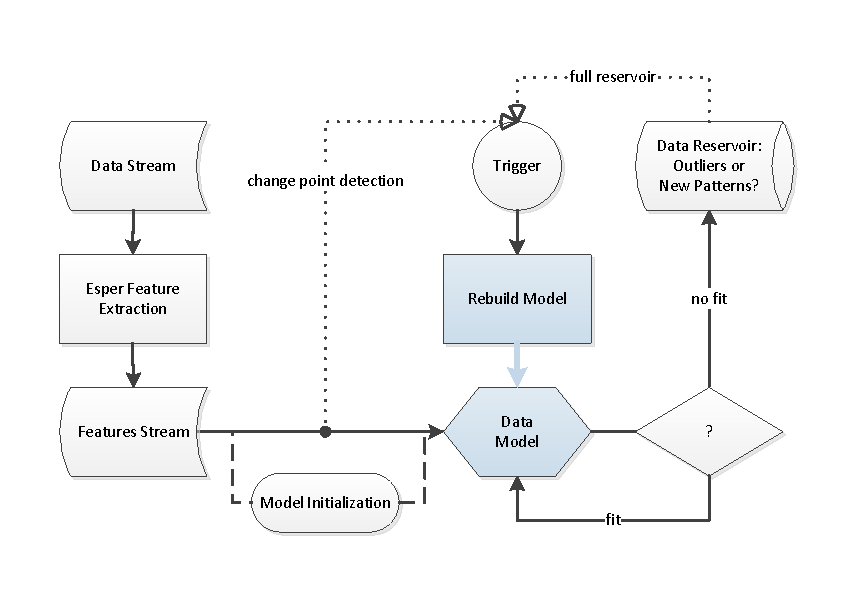
\includegraphics[width=\textwidth]{./gfx/APC_Presentation.pdf}
  \caption{Stream clustering model.\label{fig:APC}}
\end{figure}

\noindent The detailed description of outlined approach is presented in \emph{Algorithm}~\ref{alg:APC}.\\

\RestyleAlgo{boxed}
\SetAlCapSkip{1em}
\LinesNumbered
\SetCommentSty{mycommfont}
\vspace{2cm}
\begin{algorithm}[h]
  \KwData{Data stream $...x_t, x_{t+1}, x_{t+2}, ...$;number of initialization points $T$; reservoir size $r$; fit threshold $\epsilon$.}

  \tcc{Initialization}
  $m$ \leftarrow APModel($x_1, ..., x_T$)\;
  $Reservoir$ \leftarrow \{\}\;

  \tcc{Receiving data}
  \For{$t > T$}{
  Compute $e_i =$ nearest exemplar to $x_t$ \;

  \uIf{$d\left( x_t, e_i \right) < \epsilon$}{Update model $m$ \;}
  \Else{$Reservoir$ \leftarrow $x_t$\;}

  Rebuild Trigger \leftarrow ( $\left\vert{Reservoir}\right\vert > r$ || Change Point Detection on input stream )\;

  \If{Rebuild Trigger}{
    Rebuild model $m$\;
    $Reservoir$ \leftarrow \{\}\;
  }

    \caption{Streaming Affinity Propagation Clustering Algorithm.\label{alg:APC}}
    }
\end{algorithm}
\vspace{1cm}


\subsubsection{Affinity Propagation\label{sec:AfinProp}}
The predominant part of my application is \emph{Affinity Propagation} module---an unsupervised clustering algorithm adapted to data streams as described above (§\ref{sec:livestream}).\\

Imagine two dimensional clustering task. It can be described as finding \emph{clouds} of points which are similar. If we choose an Euclidean distance as our similarity measure the task is to locate areas on $\mathbb{R}^2$ plain where points lie close together.\\
Each cluster can be represented by a \emph{medoid} or a \emph{centroid}. The first is a central datum point of a ``cloud'' that \emph{belongs} to the data set; and the later is a point on a plane which describes ``centre of gravity'' of the ``cloud''.\\

Affinity Propagation is a state-of-the-art clustering solution based on concept of message passing between data points. The algorithm uses notion of distance or similarity between any two points to find centroids of clusters. To this end, it maintains two matrices: $R$---\emph{responsibility matrix} and $A$---\emph{availability matrix}. Entries $r_{ij}$ of the first one quantify how good does a datum point $x_j$ act as an exemplar for $x_i$. Matrix $A$ with elements $a_{ij}$ describes how well does $x_i$ fit to the model while being assigned to exemplar $x_j$.\\
Both matrices are initialised to $0$ and iteratively updated by passing messages between each other. Once they are ready, one can retrieve from them the most probable centroids and all points assigned to them. For more details please refer to~\citep{frey07affinitypropagation}.\\

\subsection{Data visualization}
To visualize gathered data, I wrote a separate \texttt{Python} script. It uses \texttt{CSV} repository generated by the main program to show the signal and its defined features as functions of time. It is also capable of plotting in ``re-play'' mode, where timestamps are used to model pause between plotting two adjacent points.\\
The script can also be used to scatter a plot of selected features against each other.\\

\subsection{Static clustering}
To analyse the quality of my experimental results (final stage of live clustering) I compare them with results obtained via static clustering performed on data gathered in \texttt{CSV} repository. For this purpose I use k-means, expectation-maximization, and affinity propagation algorithms. First two are implemented in \texttt{Weka} machine learning tool-kit and the last one is a part of \emph{APCluster} package for \texttt{R} language.


\section{Results}
The application is evaluated on signals produced by described above generators (see §\ref{sec:generators}). This section is supported by an example of generated \emph{noisy sine wave} showed in \emph{Figure}~\ref{fig:signal}.\\

\begin{figure}[htbp]
  \centering
  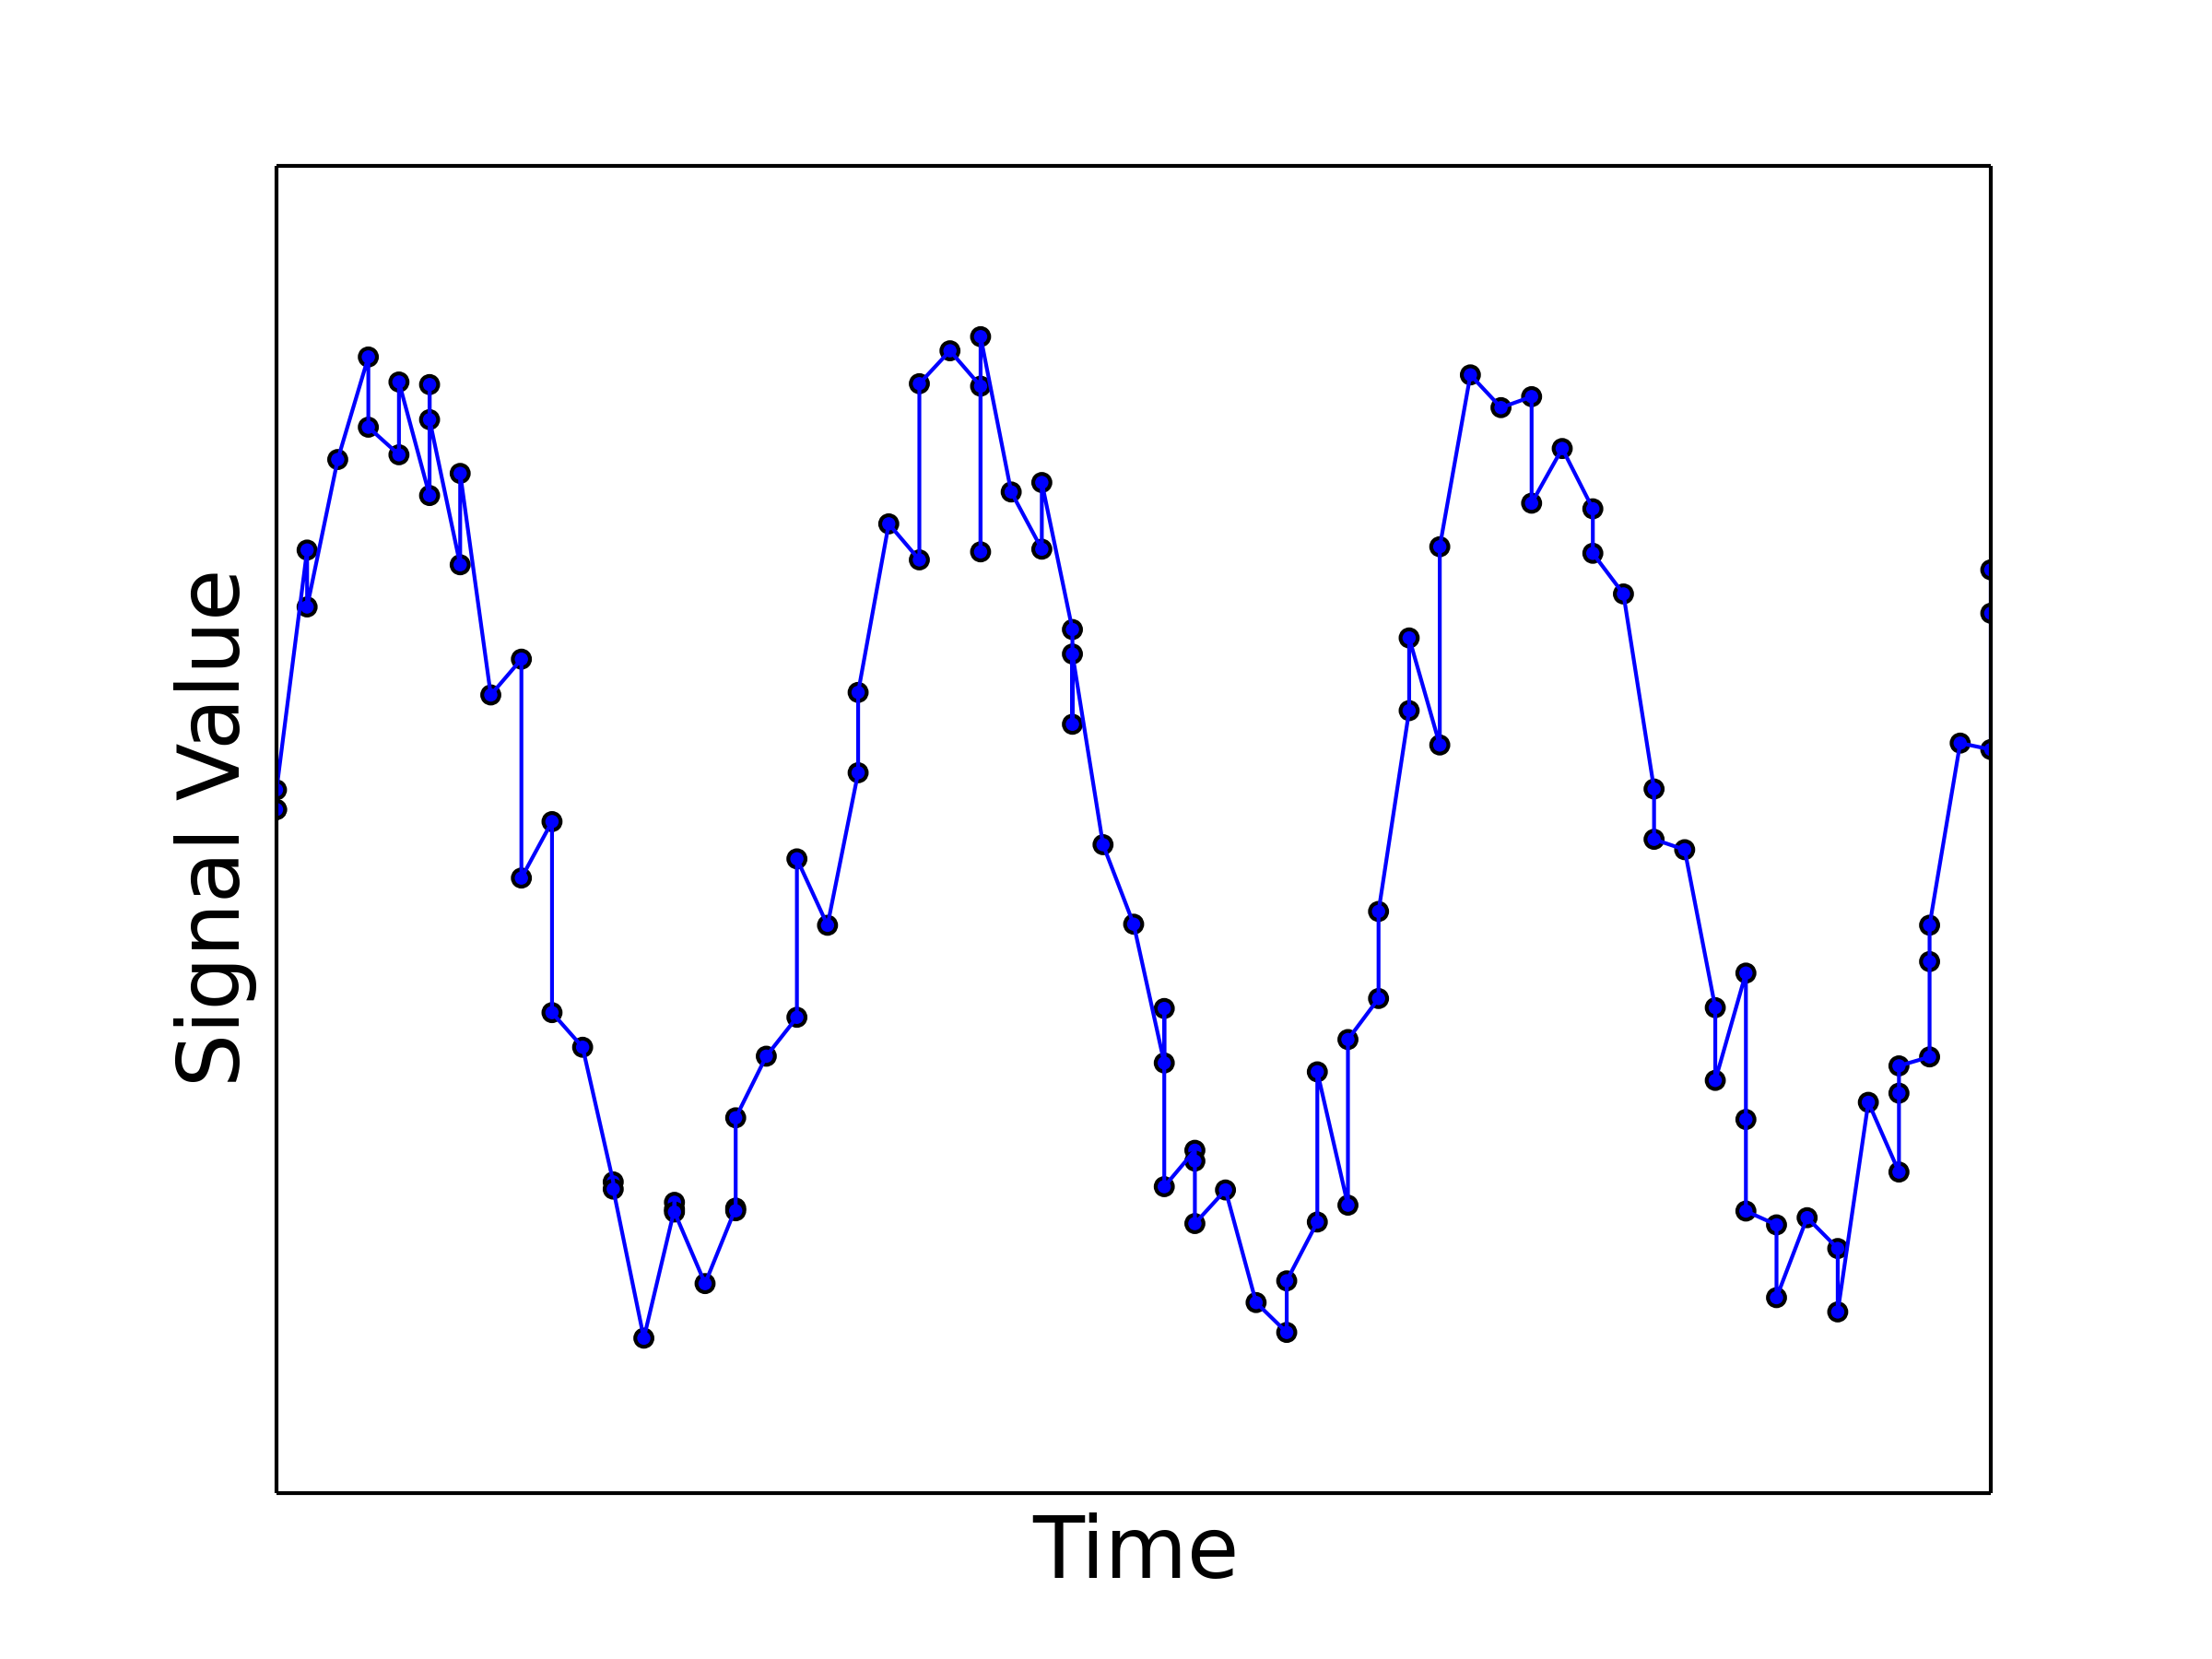
\includegraphics[width=.7\textwidth]{./gfx/feature5.png}
  \caption{Generated signal sample---noisy sine wave.\label{fig:signal}}
\end{figure}

The second step in processing is feature extraction. The sample of such features, extracted in \emph{60 seconds sliding time window}, represented by \emph{average}, \emph{standard deviation}, and \emph{5-Lag} are presented in \emph{Figure}~\ref{fig:features}.\\

\begin{figure}[htbp]
  \centering
  \begin{subfigure}[b]{0.49\textwidth}
    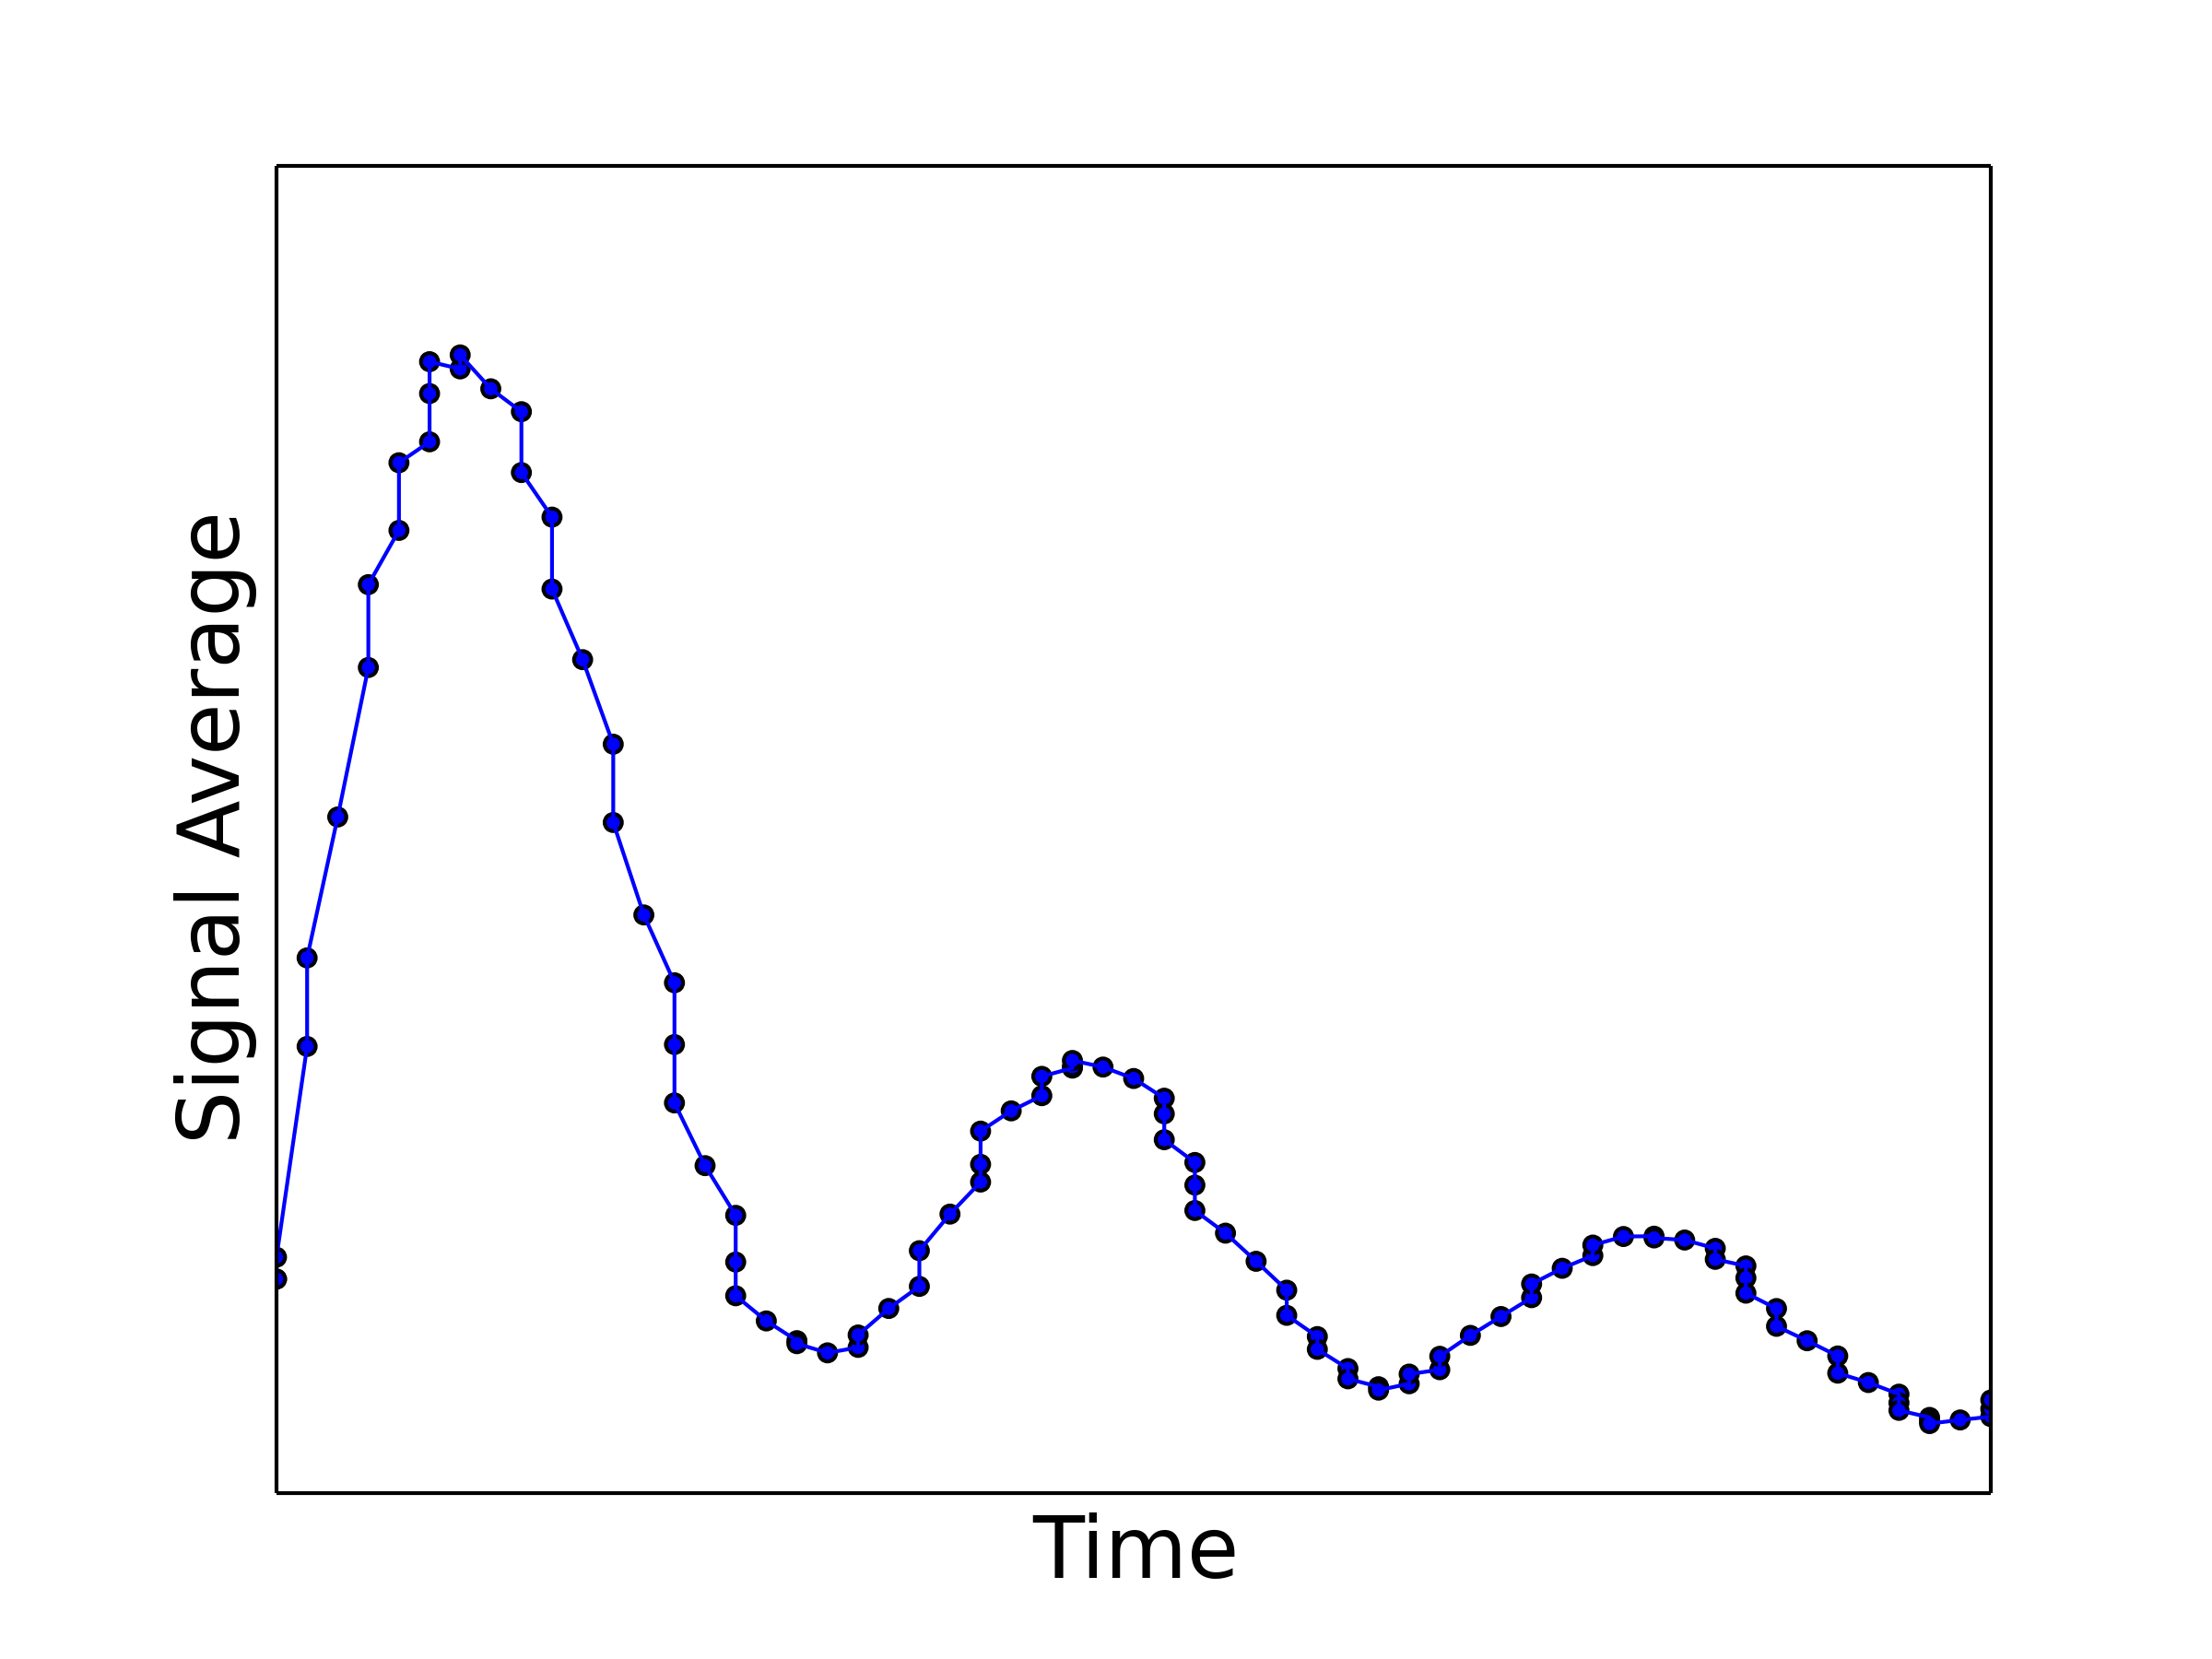
\includegraphics[width=\textwidth]{./gfx/feature1-1.png}
    \caption{Signal average in time.\label{fig:average}}
  \end{subfigure}%
  ~ %add desired spacing between images, e. g. ~, \quad, \qquad, \hfill etc.
    %(or a blank line to force the subfigure onto a new line)
  \begin{subfigure}[b]{0.49\textwidth}
    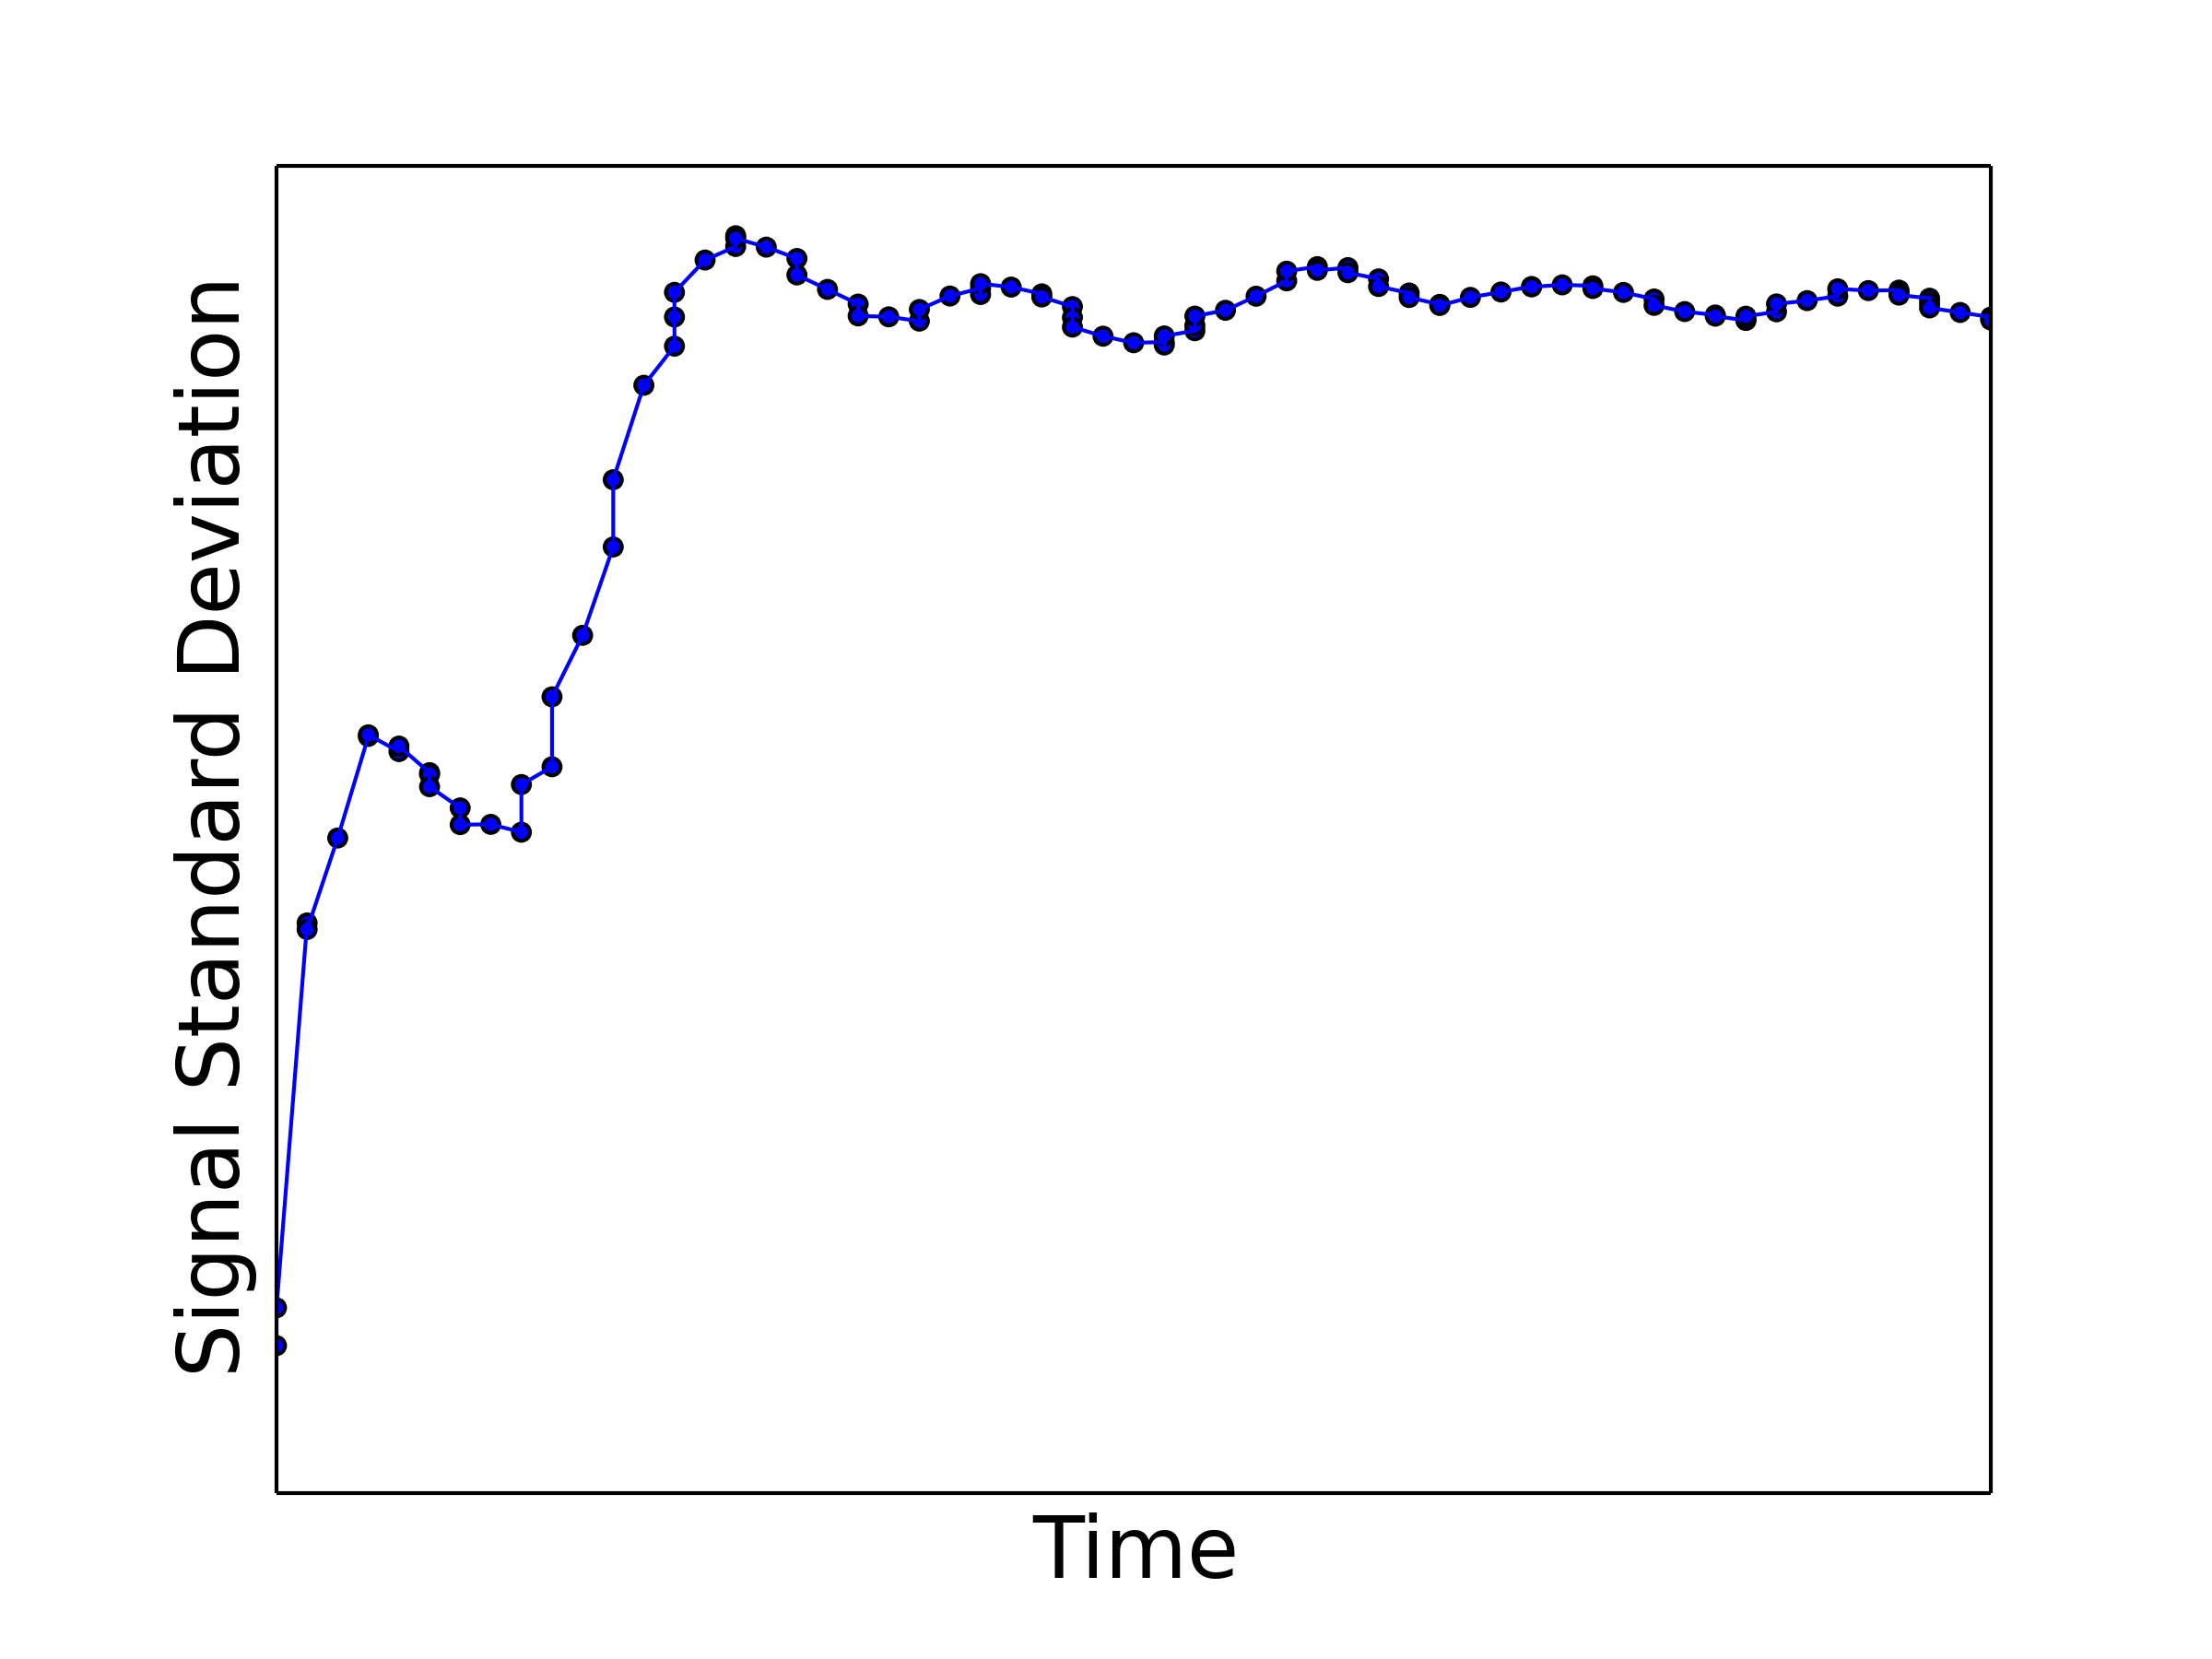
\includegraphics[width=\textwidth]{./gfx/feature2-1.png}
    \caption{Signal standard deviation in time.\label{fig:standarddeviation}}
  \end{subfigure}
  ~ %add desired spacing between images, e. g. ~, \quad, \qquad, \hfill etc.
    %(or a blank line to force the subfigure onto a new line)
  \begin{subfigure}[b]{0.49\textwidth}
    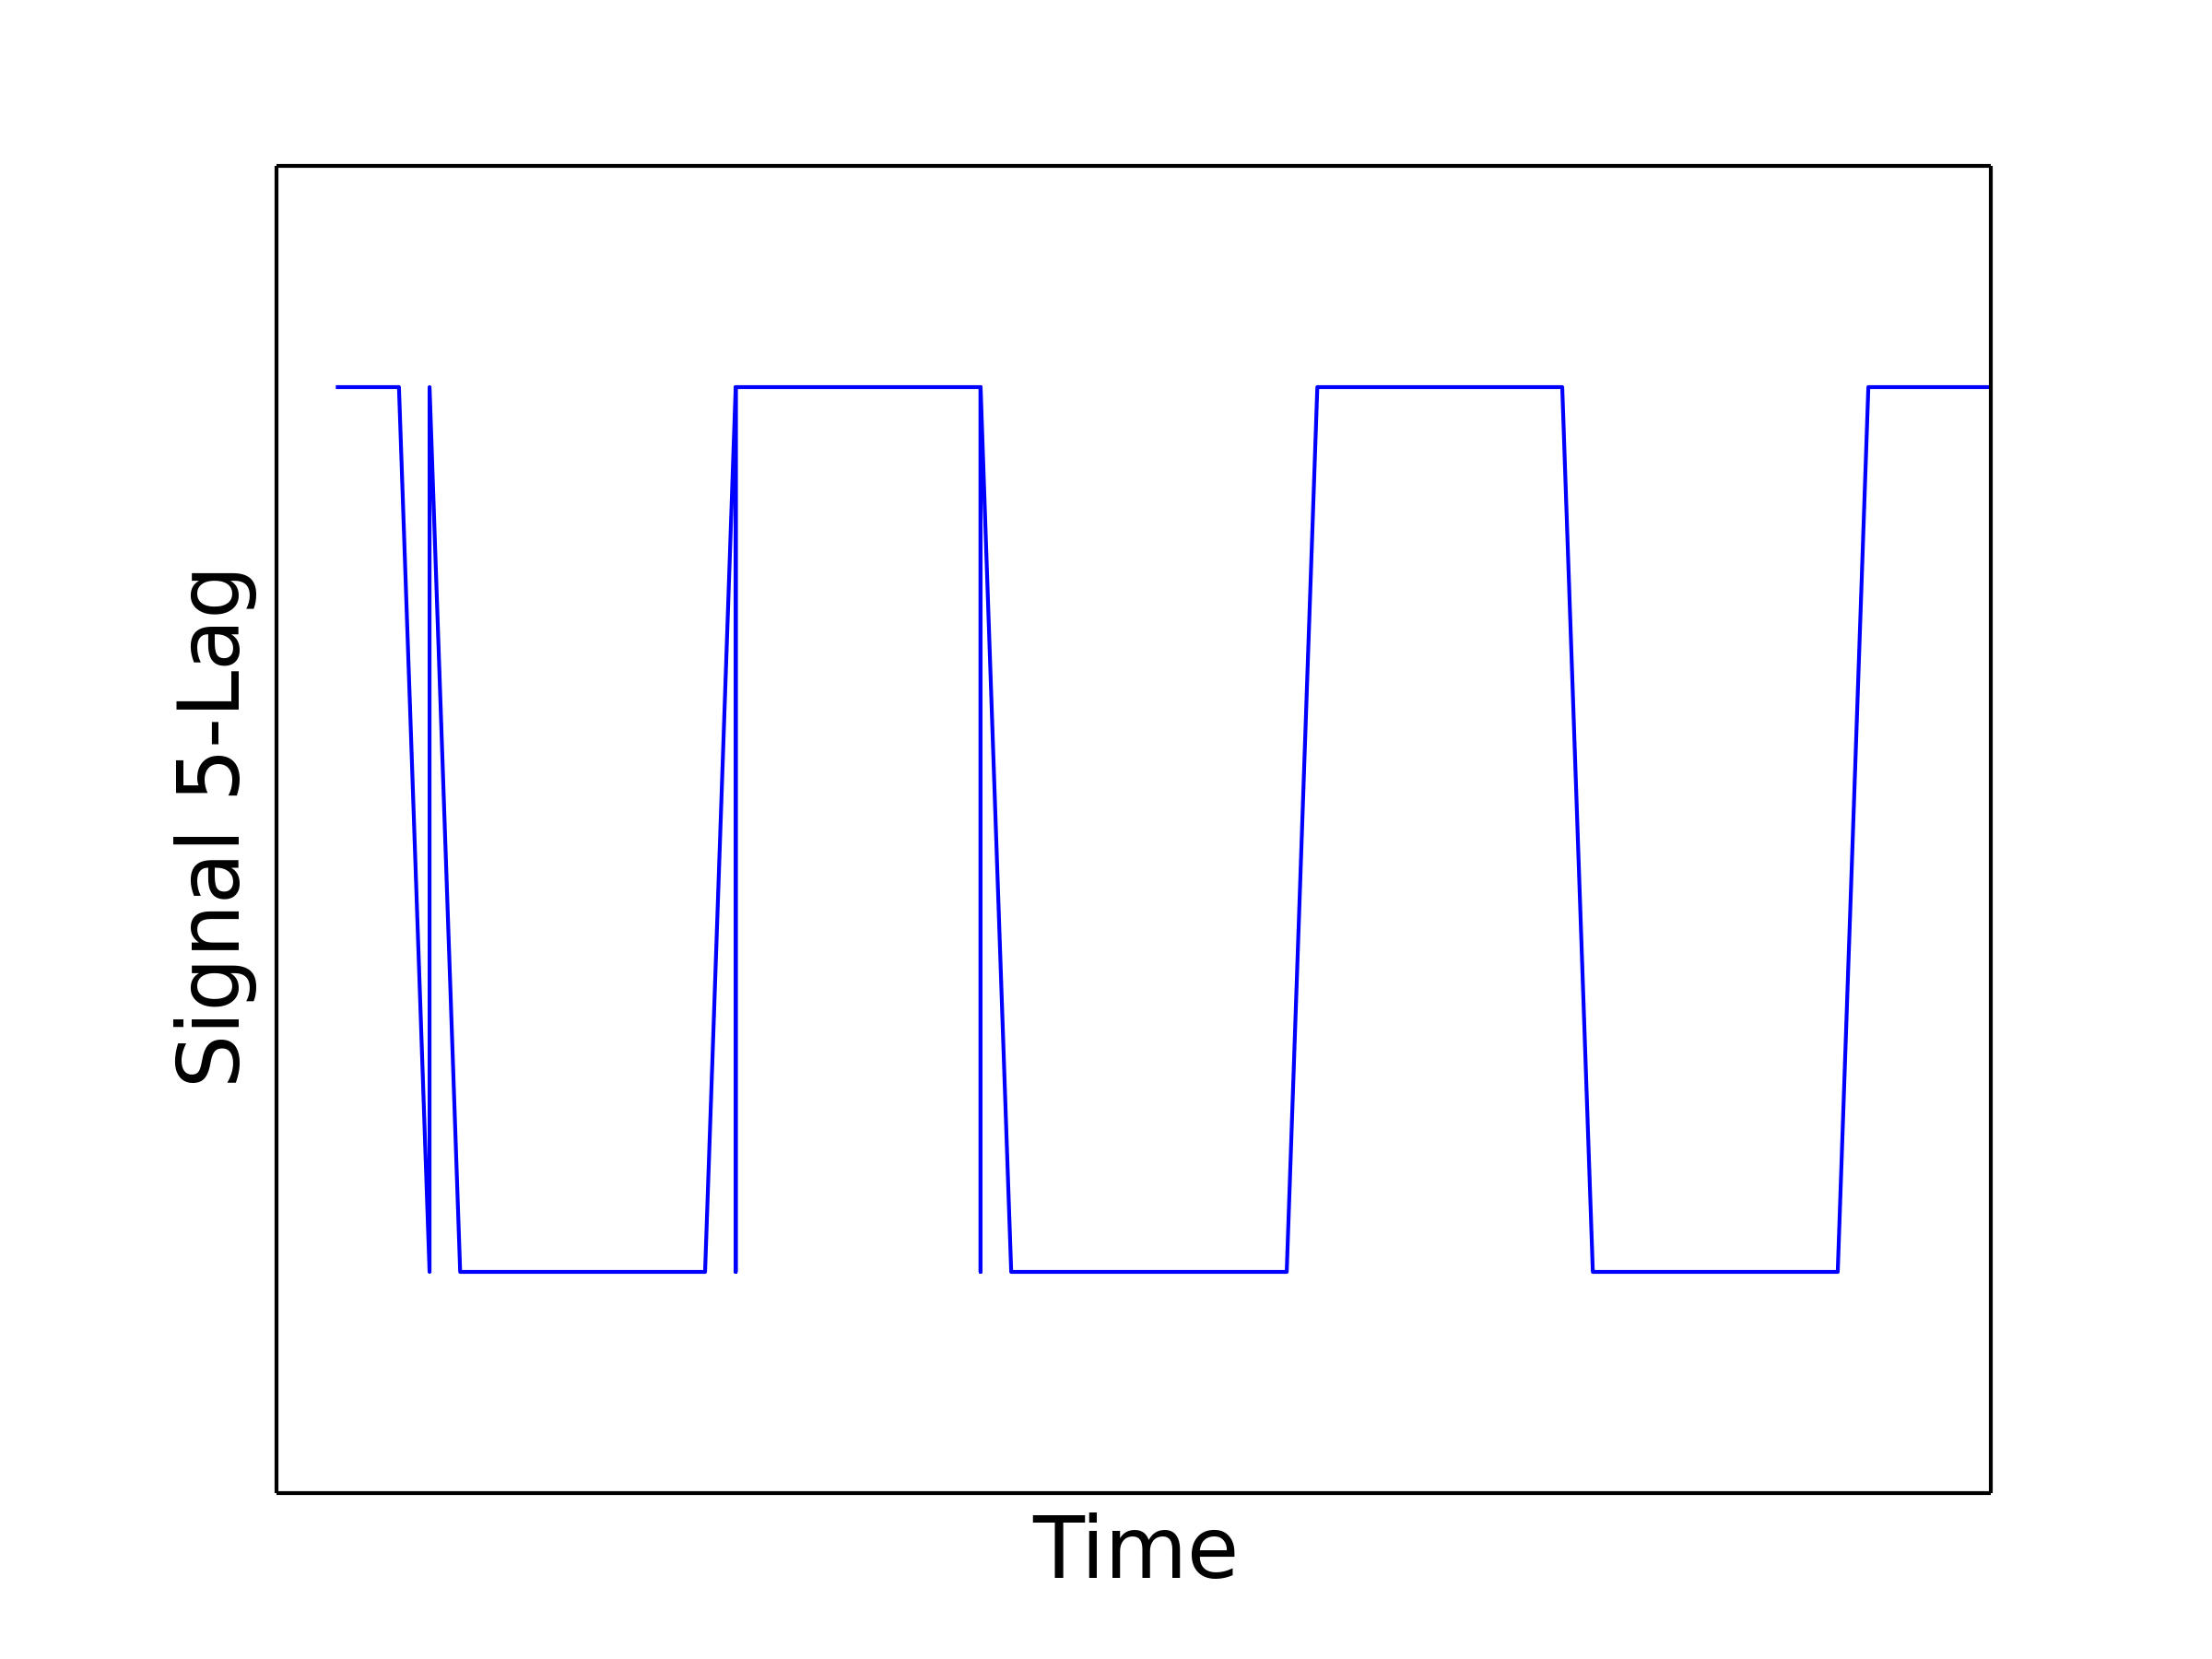
\includegraphics[width=\textwidth]{./gfx/feature3-1.png}
    \caption{Signal $5$-Lag in time.\label{fig:lag}}
  \end{subfigure}
  \caption{Features extracted form signal.\label{fig:features}}
\end{figure}

Finally, affinity propagation clustering runs in the background to classify incoming points. Sample results of clustering can be seen in \emph{Figure}~\ref{fig:clustering}, where each colour corresponds to separate cluster.\\
The main idea behind clustering of signals is to either raise an alarm in case of abnormal behavior or recognize the current status of signal. The first one can be understood as points appearing outside of main cluster (see \emph{Figures}~\ref{fig:Caverage}~and~\ref{fig:Cstandarddeviation}), and the later as current status of signal (see \emph{Figure}~\ref{fig:Clag}).\\
In case of sine wave the first one could be sudden change of \emph{period} or stretch in $y$-axis dimension, and the later classification on:
\begin{itemize}
  \item increasing---decreasing,
  \item positive---negative,
  \item high---low.
\end{itemize}

\begin{figure}[htbp]
  %add desired spacing between images, e. g. ~, \quad, \qquad, \hfill etc.
  %(or a blank line to force the subfigure onto a new line)
  \centering
  \begin{subfigure}[b]{0.49\textwidth}
    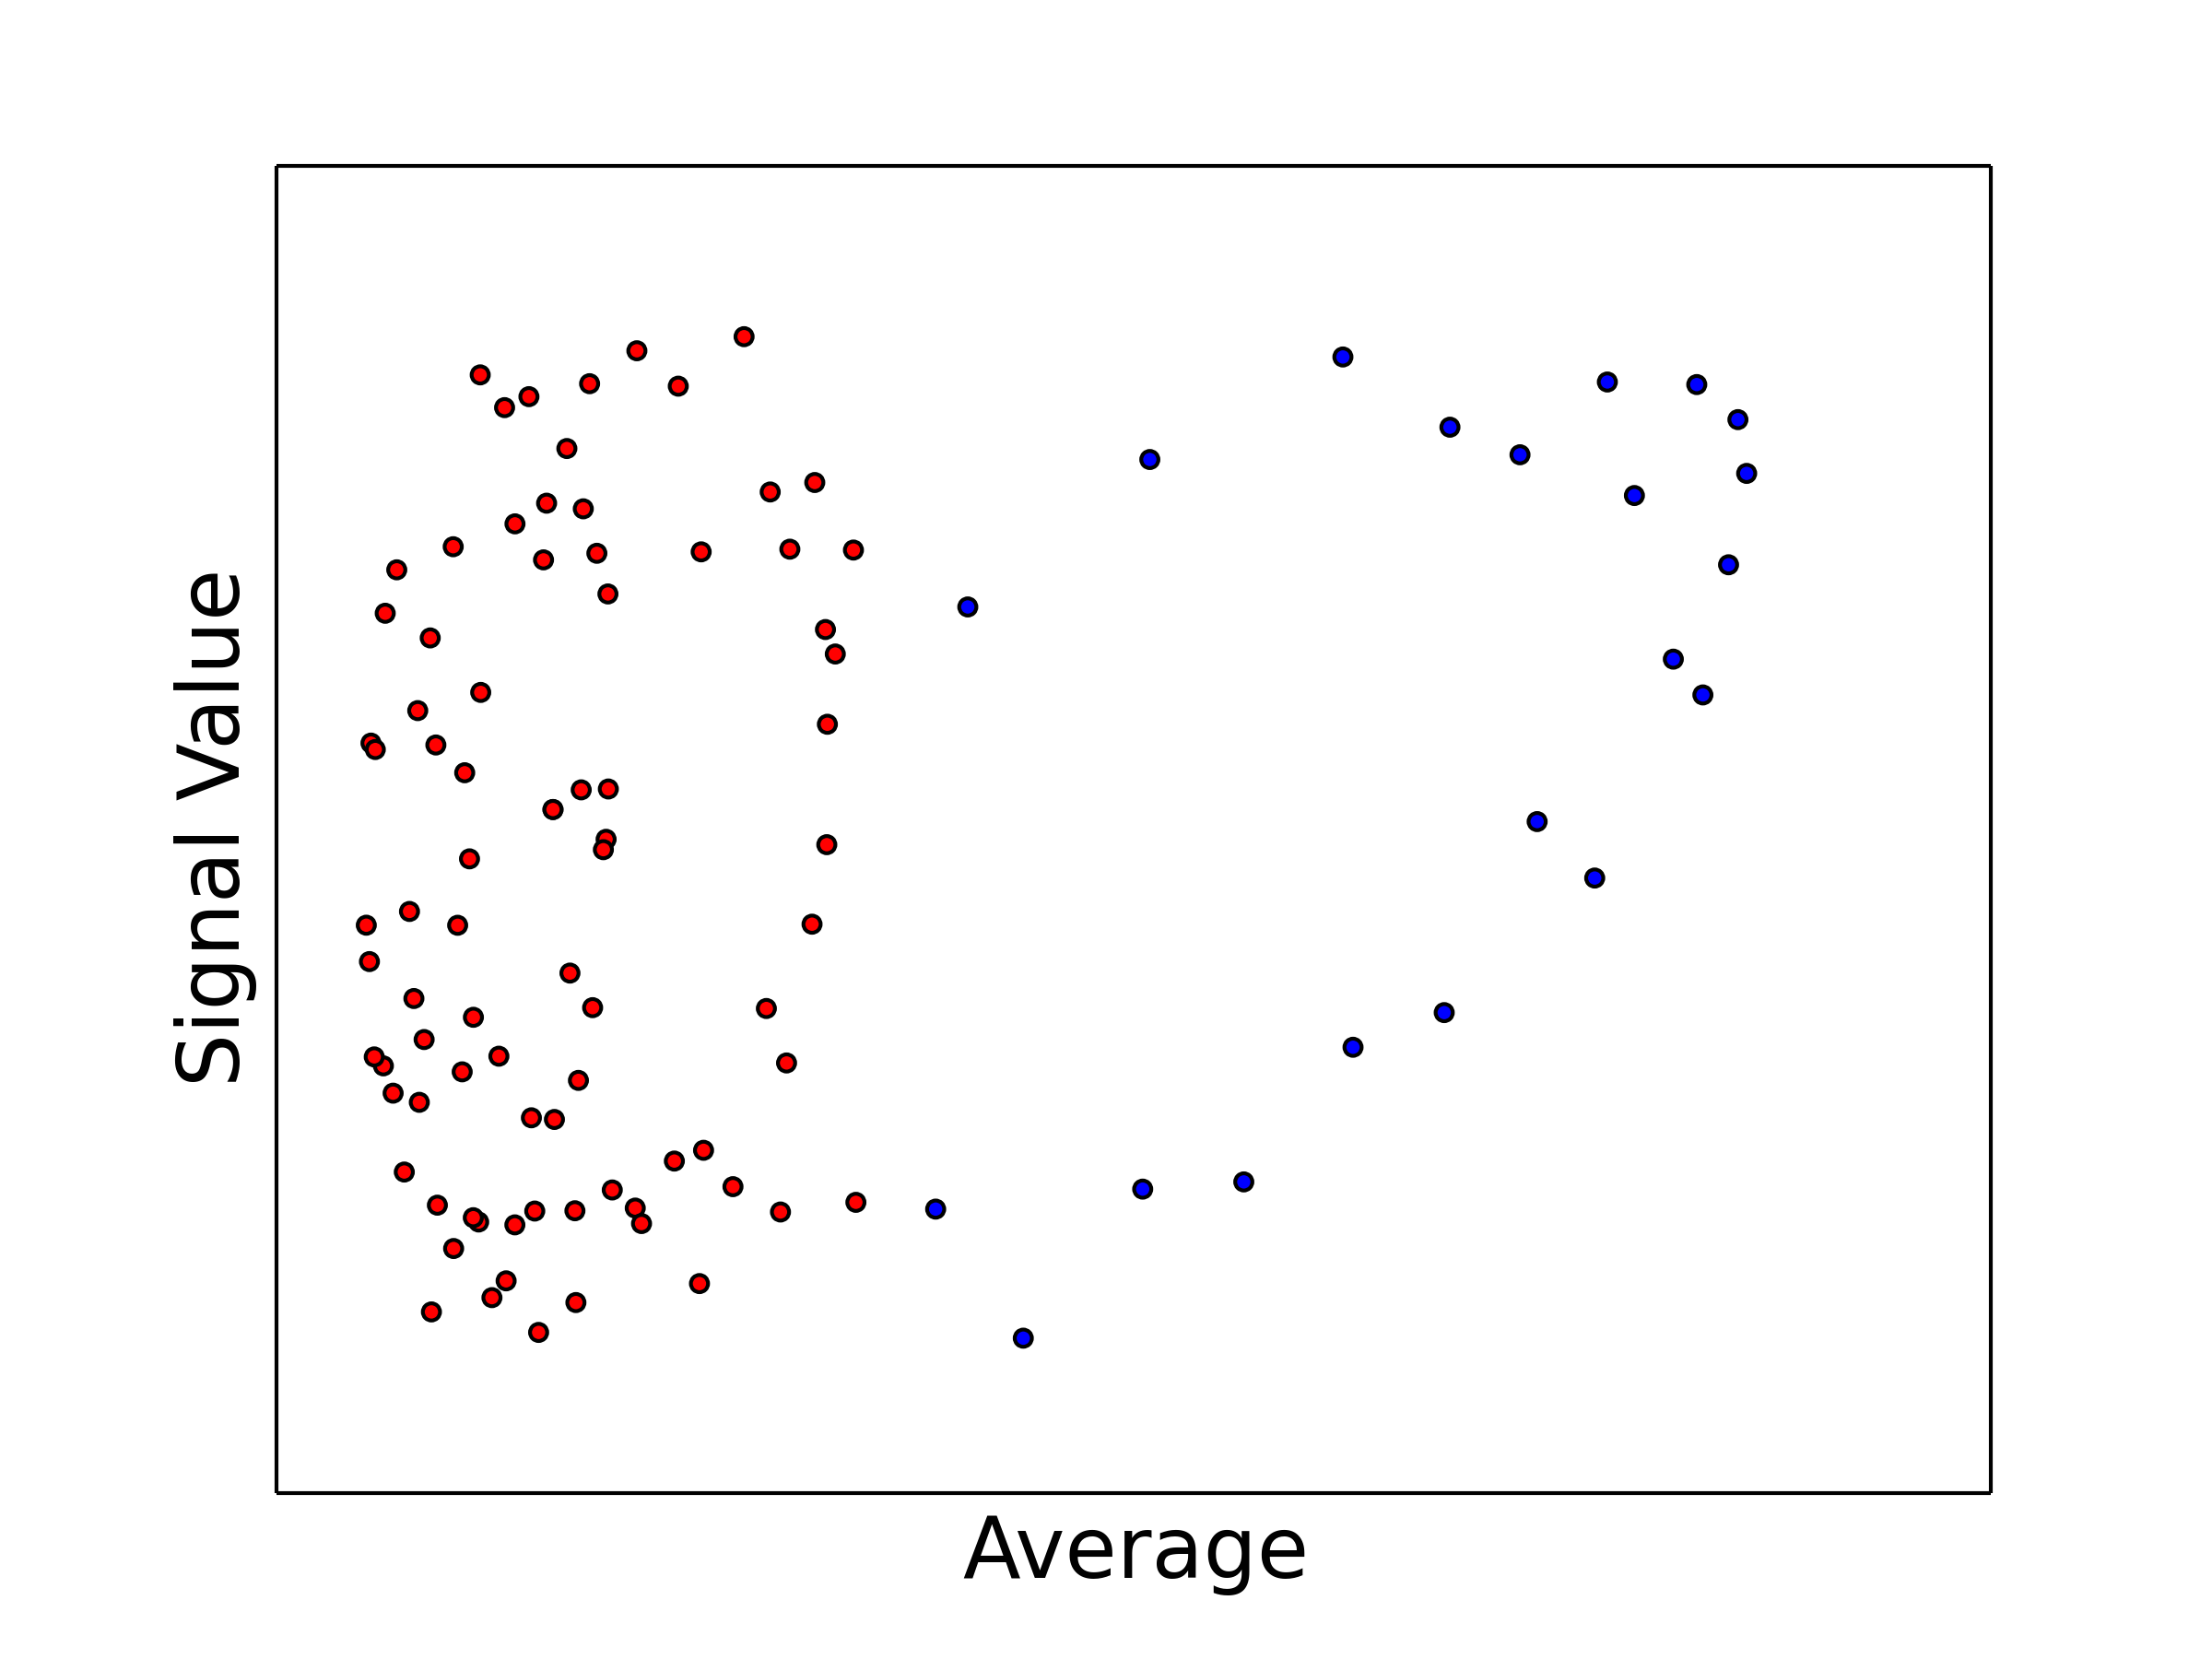
\includegraphics[width=\textwidth]{./gfx/f1f5.png}
    \caption{Average clustering.\label{fig:Caverage}}
  \end{subfigure}%
  \hfill
  \begin{subfigure}[b]{0.49\textwidth}
    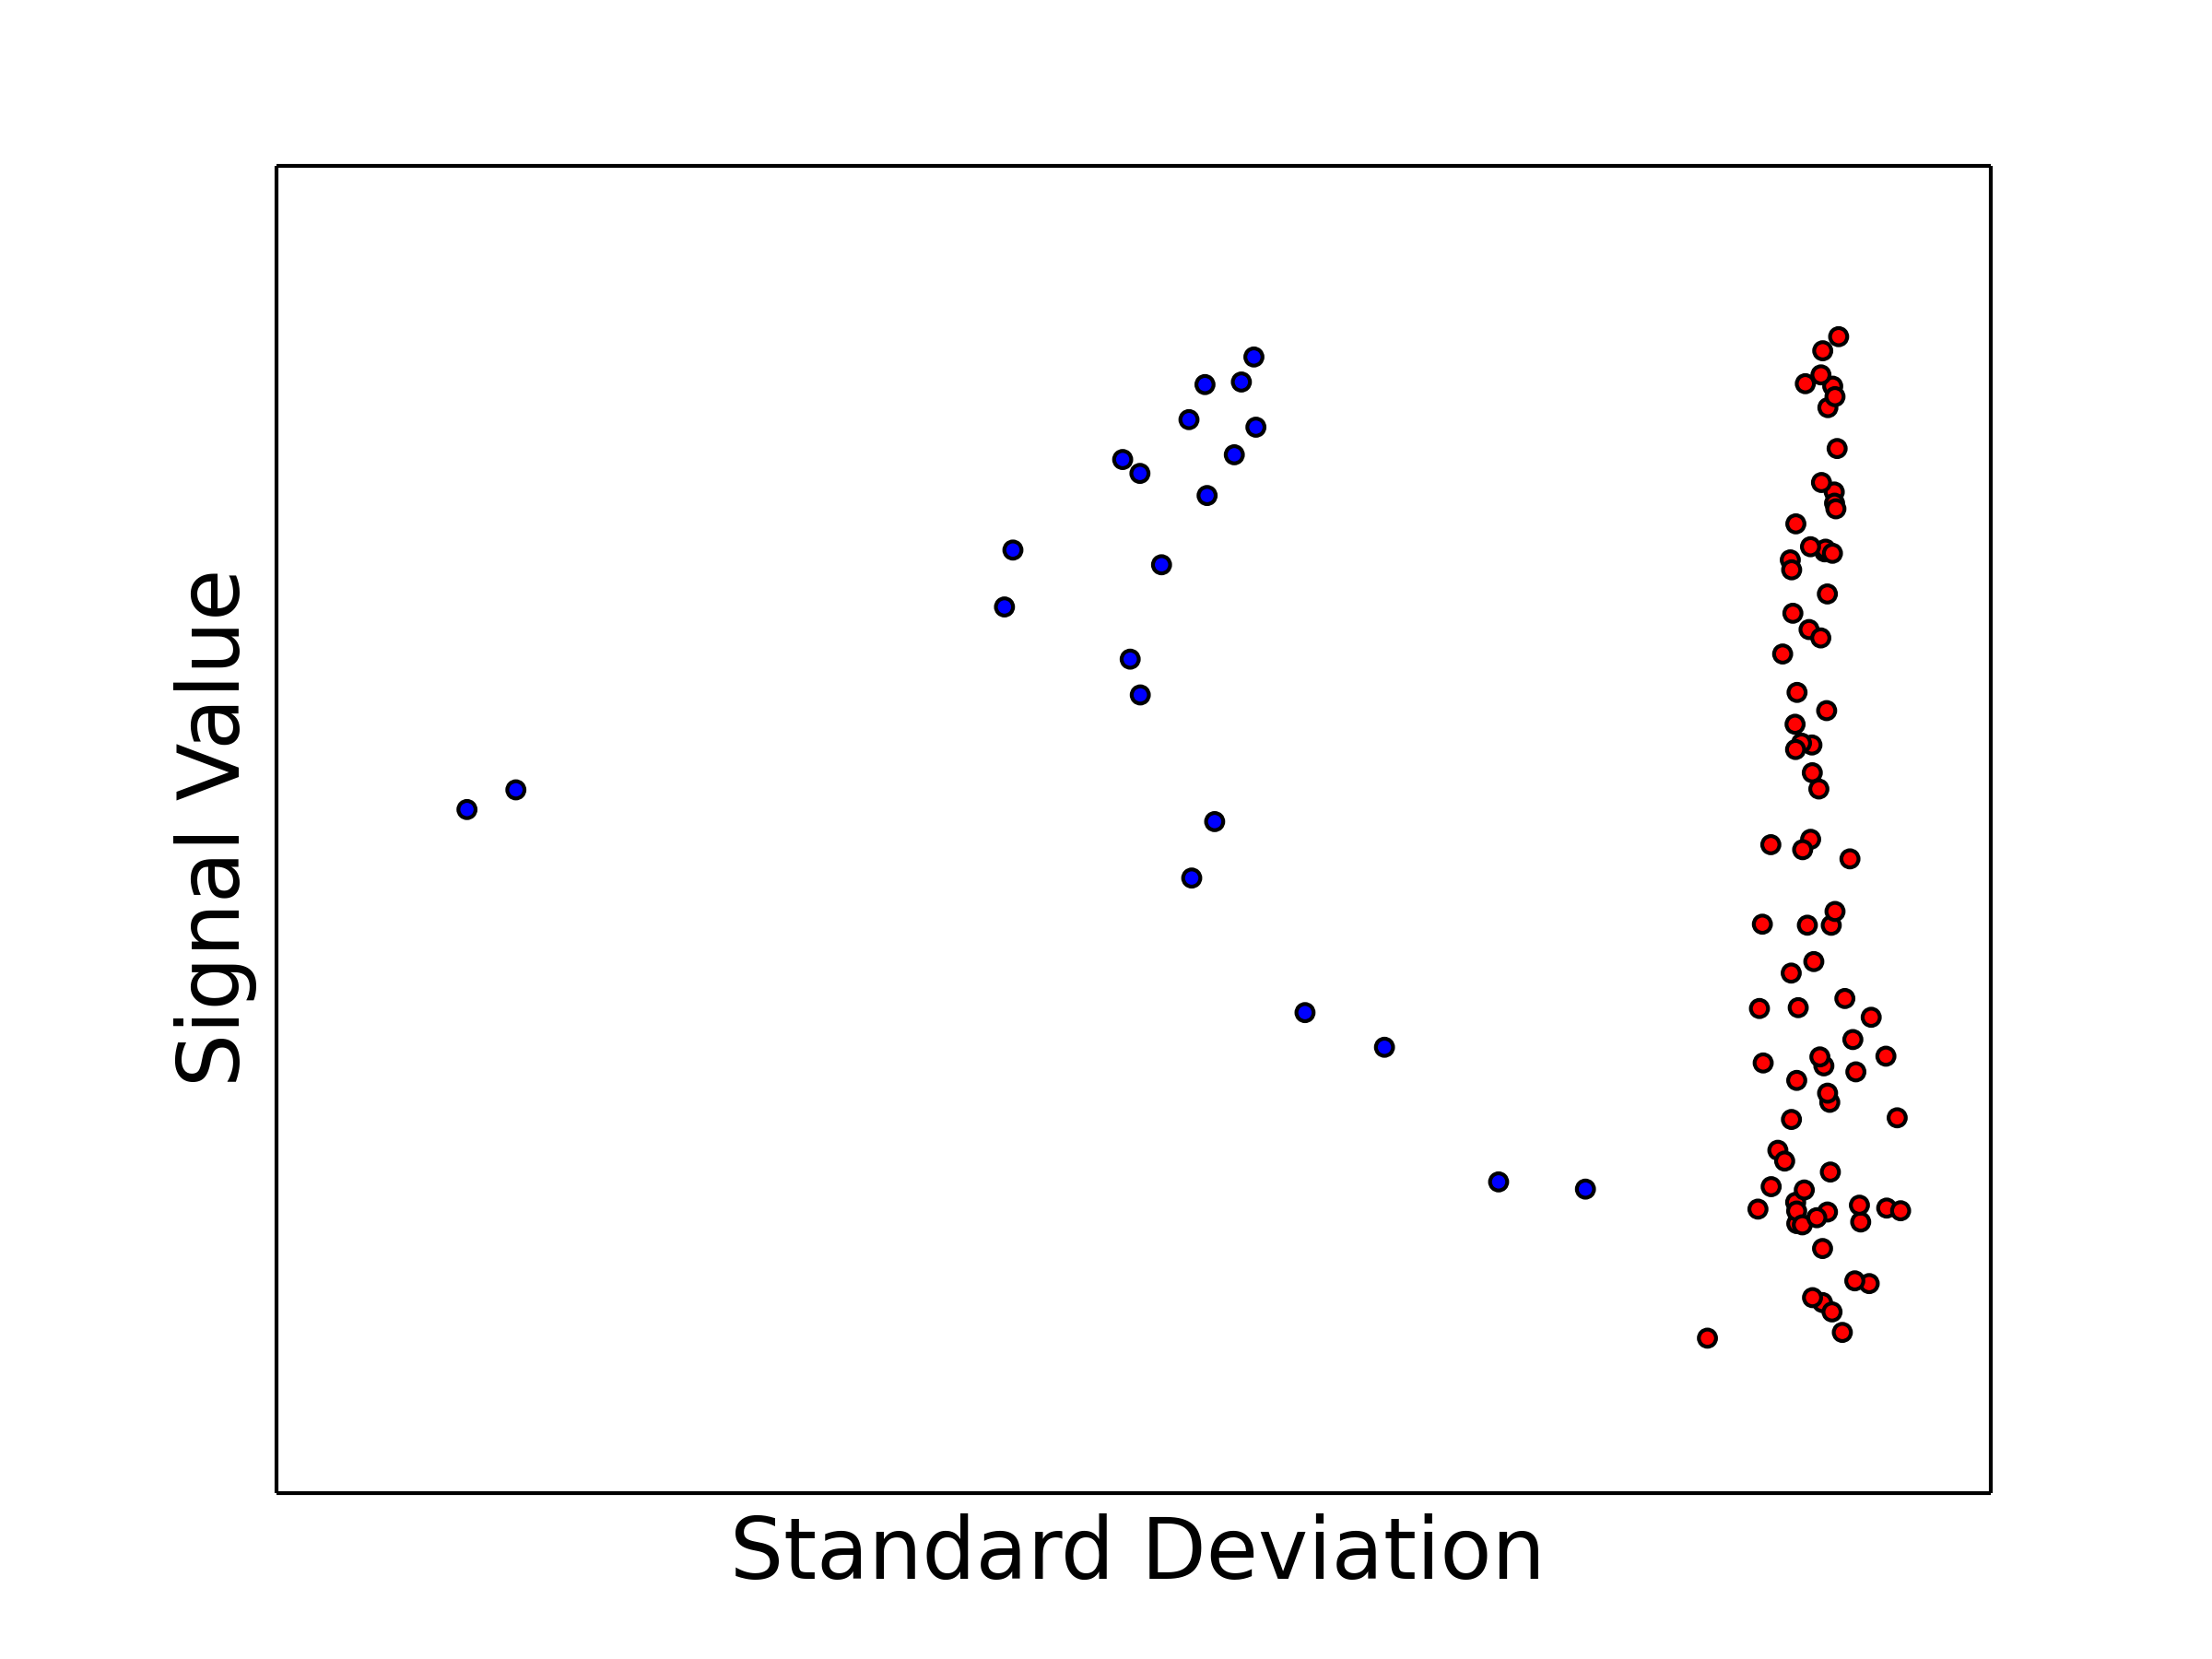
\includegraphics[width=\textwidth]{./gfx/f2f5.png}
    \caption{Standard deviation clustering.\label{fig:Cstandarddeviation}}
  \end{subfigure}

  \begin{subfigure}[b]{0.49\textwidth}
    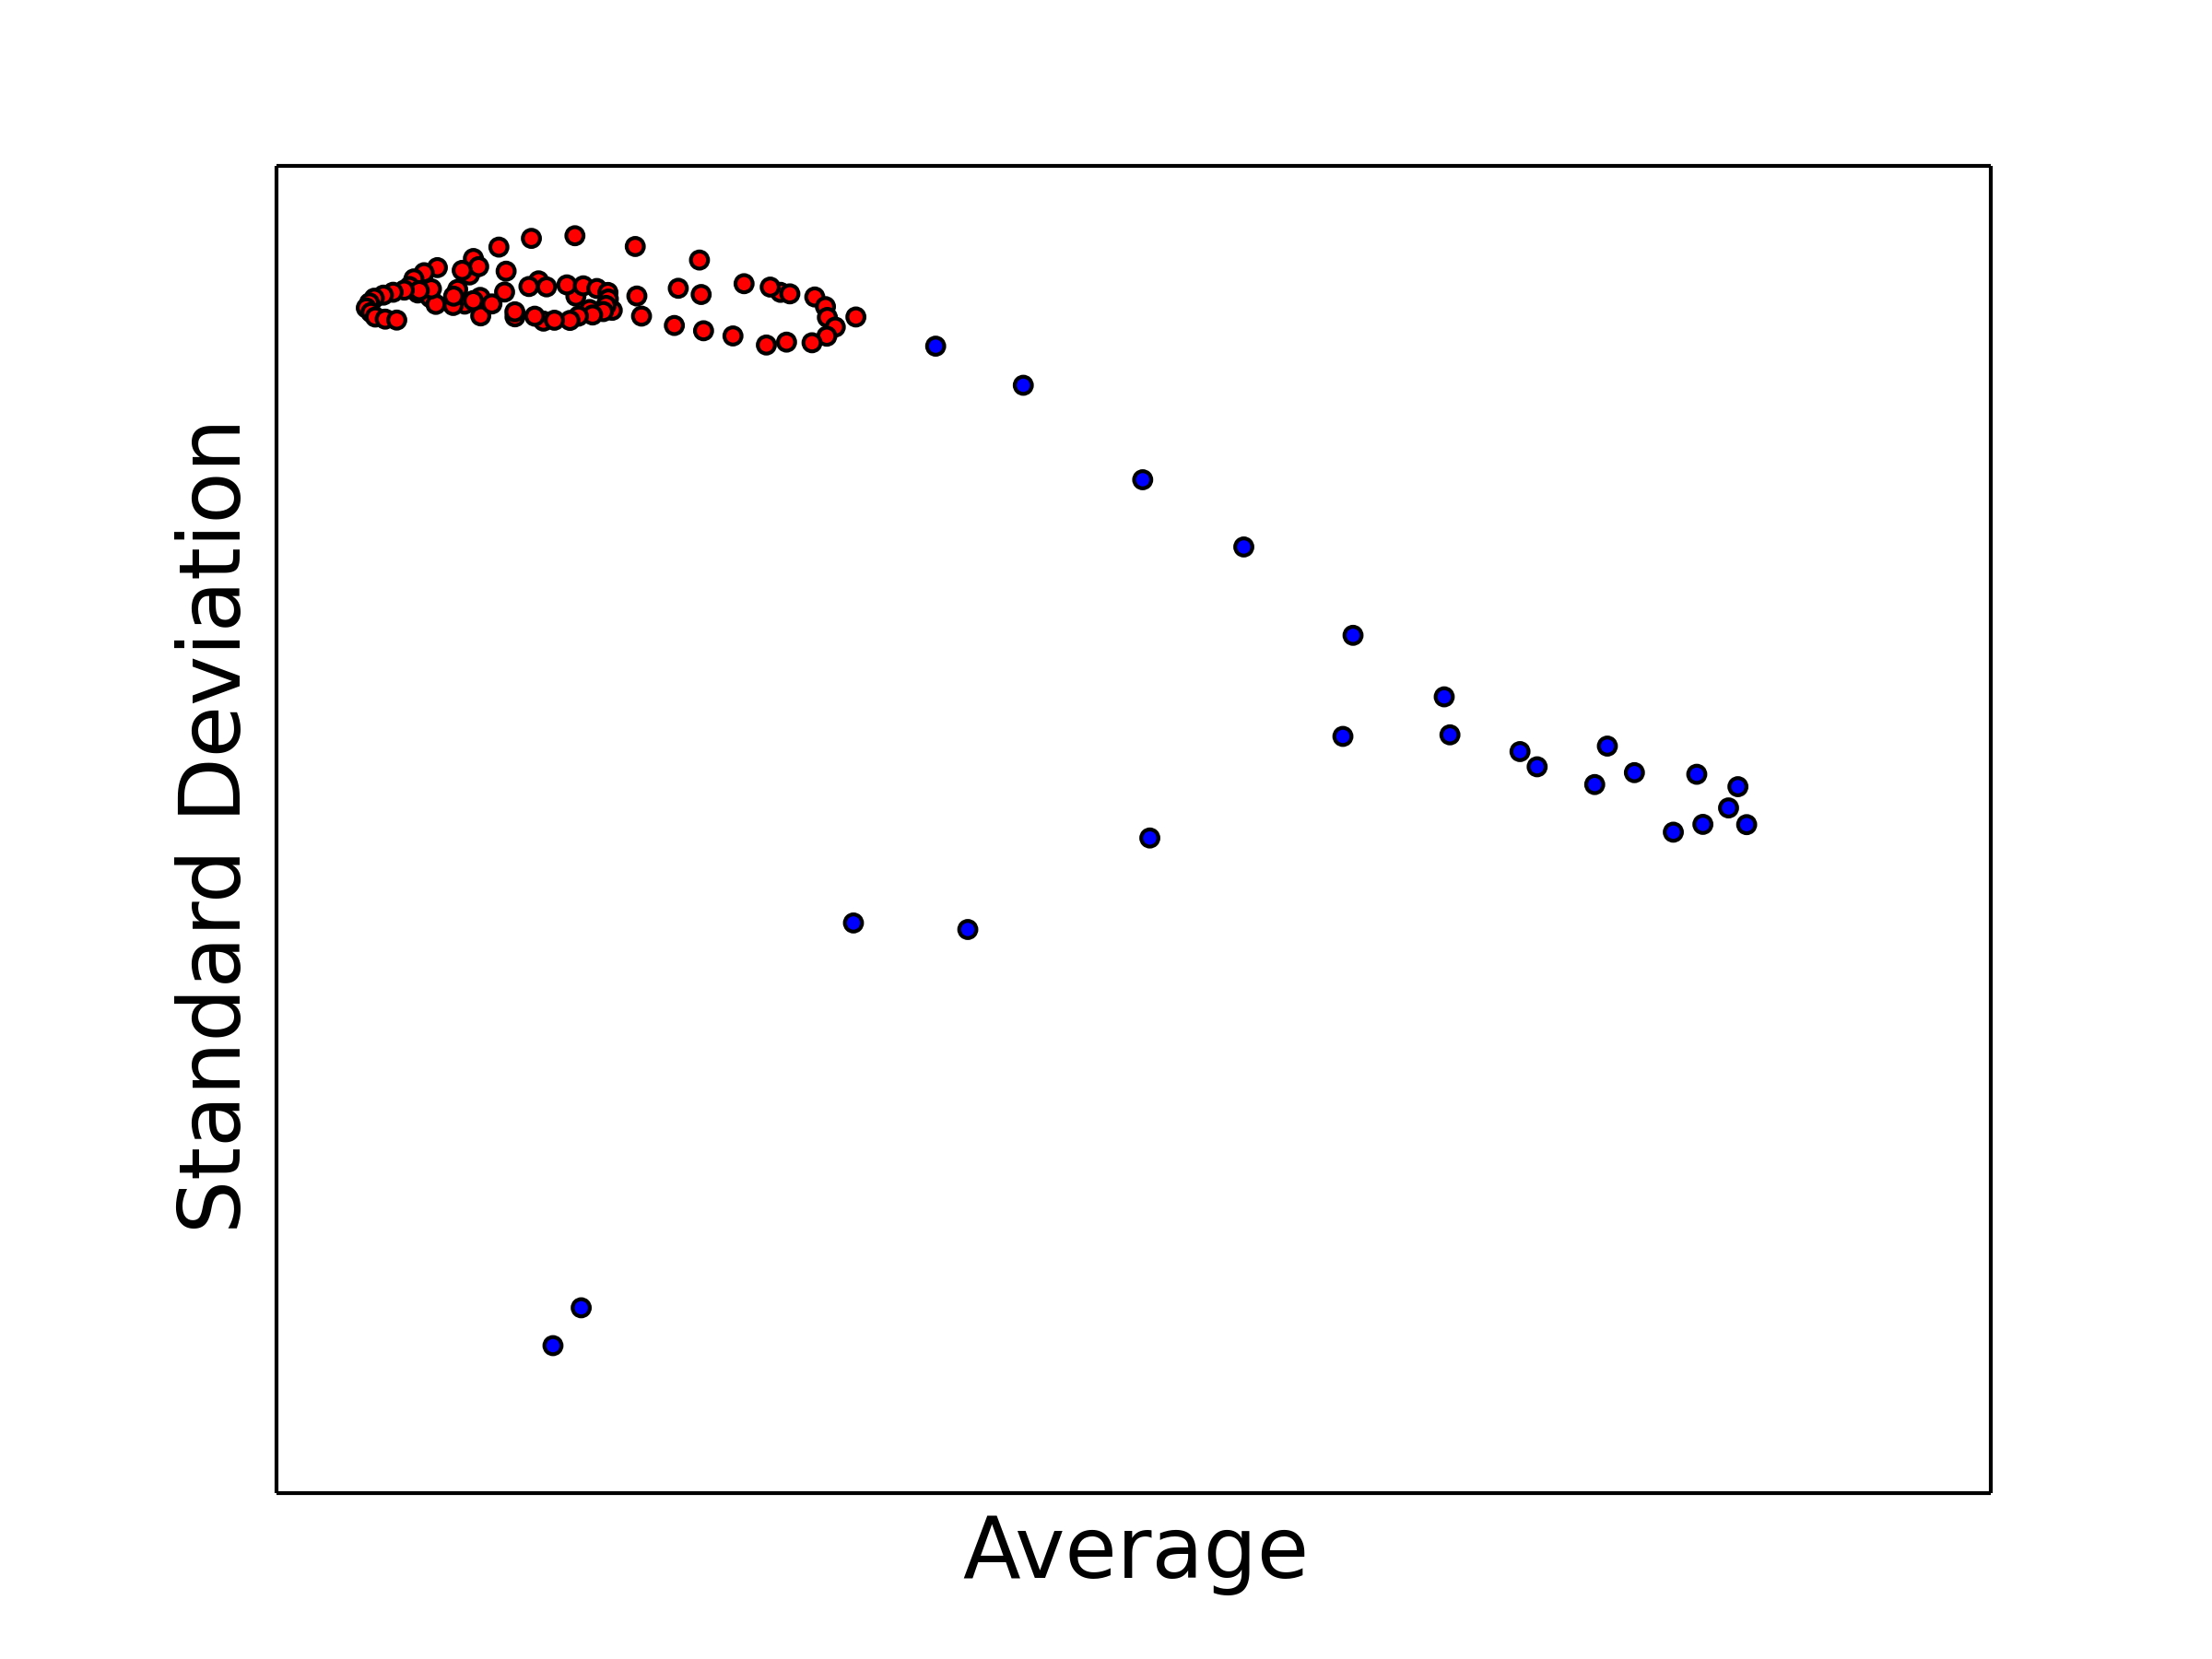
\includegraphics[width=\textwidth]{./gfx/f1f2.png}
    \caption{Average---Standard Deviation clustering.\label{fig:Cavgstd}}
  \end{subfigure}
  \hfill
  \begin{subfigure}[b]{0.49\textwidth}
    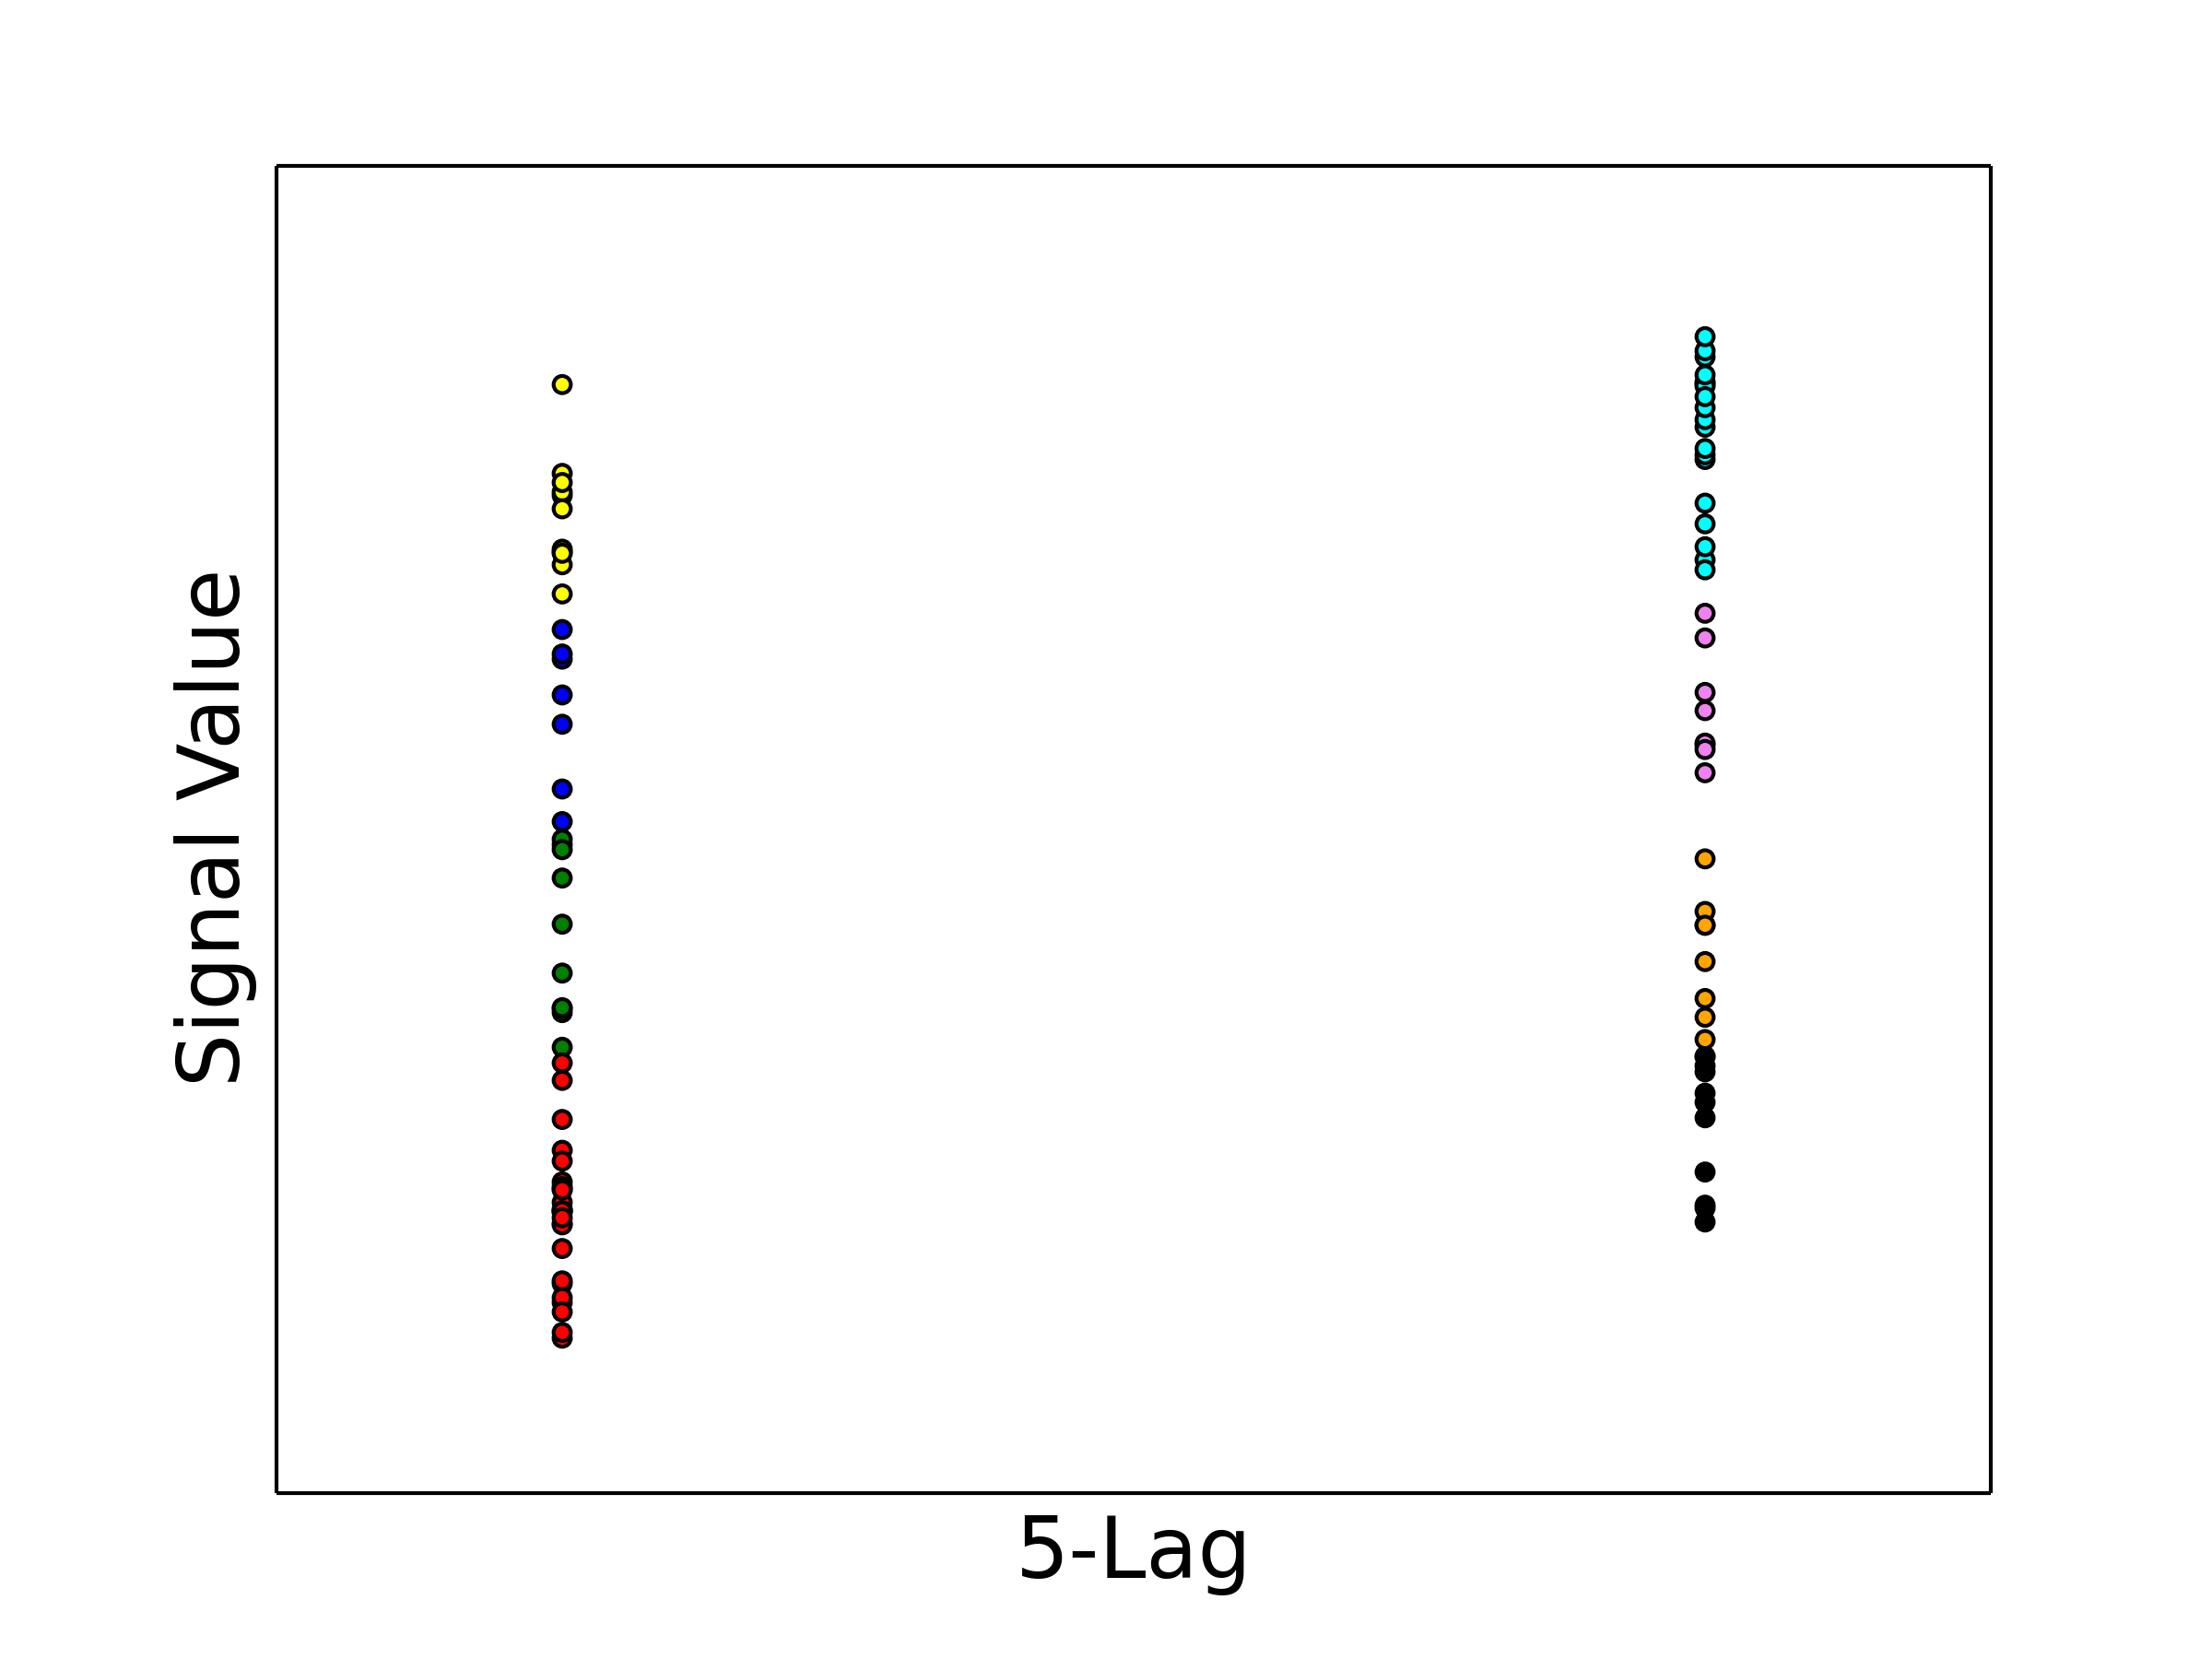
\includegraphics[width=\textwidth]{./gfx/f4f5.png}
    \caption{$5$-Lag clustering.\label{fig:Clag}}
  \end{subfigure}

  \caption{Signal clustering based on extracted features.\label{fig:clustering}}
\end{figure}

Sample ``fault'' clustering can be seen in \emph{Figures}~\ref{fig:Caverage},~\ref{fig:Cstandarddeviation},~and~\ref{fig:Cavgstd}. In all of these graphs we consider \emph{\textcolor{red}{red}} as ``healthy'' clusters, and \emph{\textcolor{blue}{blue}} as ``suspicious''.\\
It suffices to say, that if new-coming points are assigned to first the system works smoothly, once stream is being shifted towards blue zone the alarm is raised.\\

\emph{Figure}~\ref{fig:Clag} shows perfect signal recognition clustering, where each colour corresponds to combination of listed above signal states e.g.\ \emph{\textcolor{darkgreen}{green}} is \emph{decreasing-negative-low}.

\subsection{Static clustering comparison}
To benchmark above results I used static clustering on data repository created by one run of program. The algorithms are: \emph{k-means}, \emph{EM}, and \emph{Affinity Propagation}; first two implemented in \texttt{WEKA} machine learning package, and the last being package for \texttt{R} language. The choice the first one is motivated by its simplicity and popularity, nevertheless it demands fixing number of clusters therefore its application in our case is not realistic. Two later ones do not need aforementioned parameter hence are more suitable for my approach.\\


\begin{figure}[htbp]
  \centering
  \begin{subfigure}[b]{0.32\textwidth}
    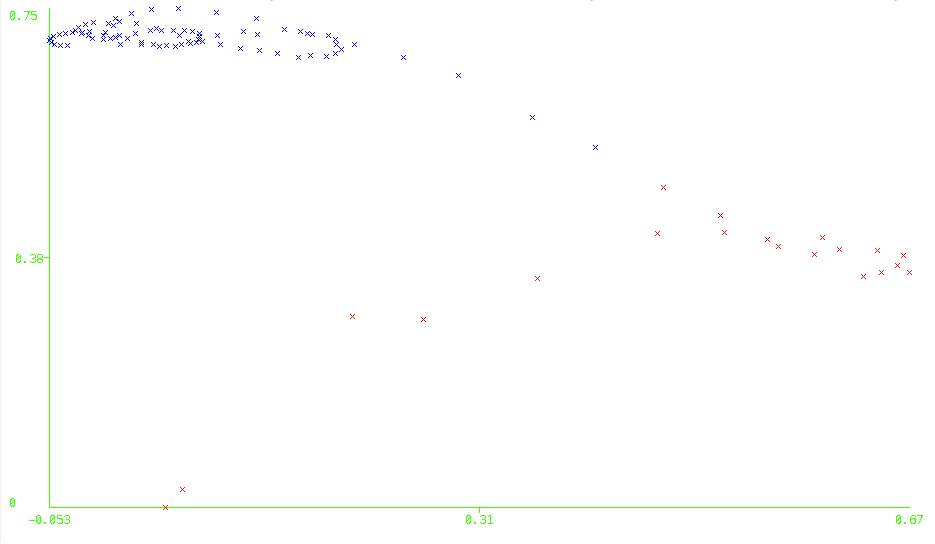
\includegraphics[width=\textwidth]{./gfx/km12.png}
    \caption{2-means clustering.\label{fig:avgstd:km}}
  \end{subfigure}
  \hfill
  \begin{subfigure}[b]{0.32\textwidth}
    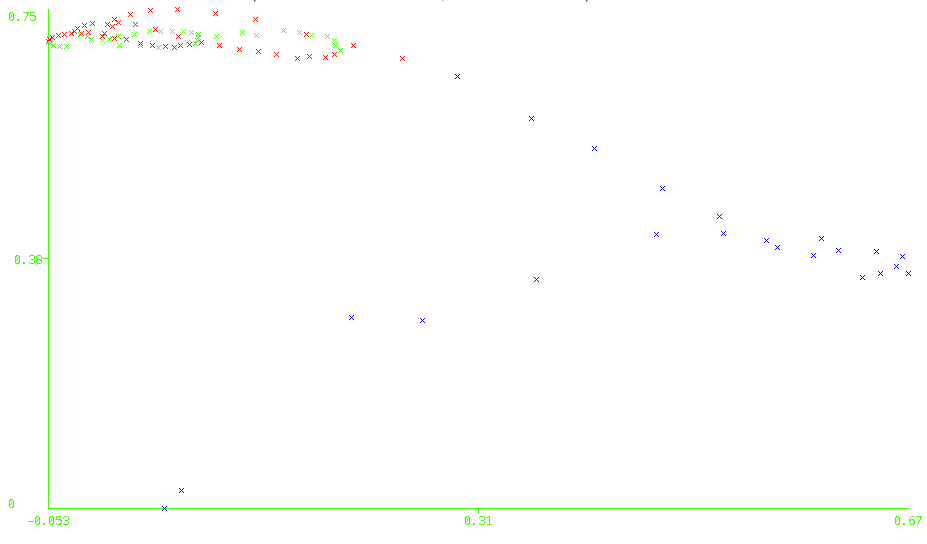
\includegraphics[width=\textwidth]{./gfx/em12.png}
    \caption{EM clustering.\label{fig:avgstd:em}}
  \end{subfigure}
  \hfill
  \begin{subfigure}[b]{0.32\textwidth}
    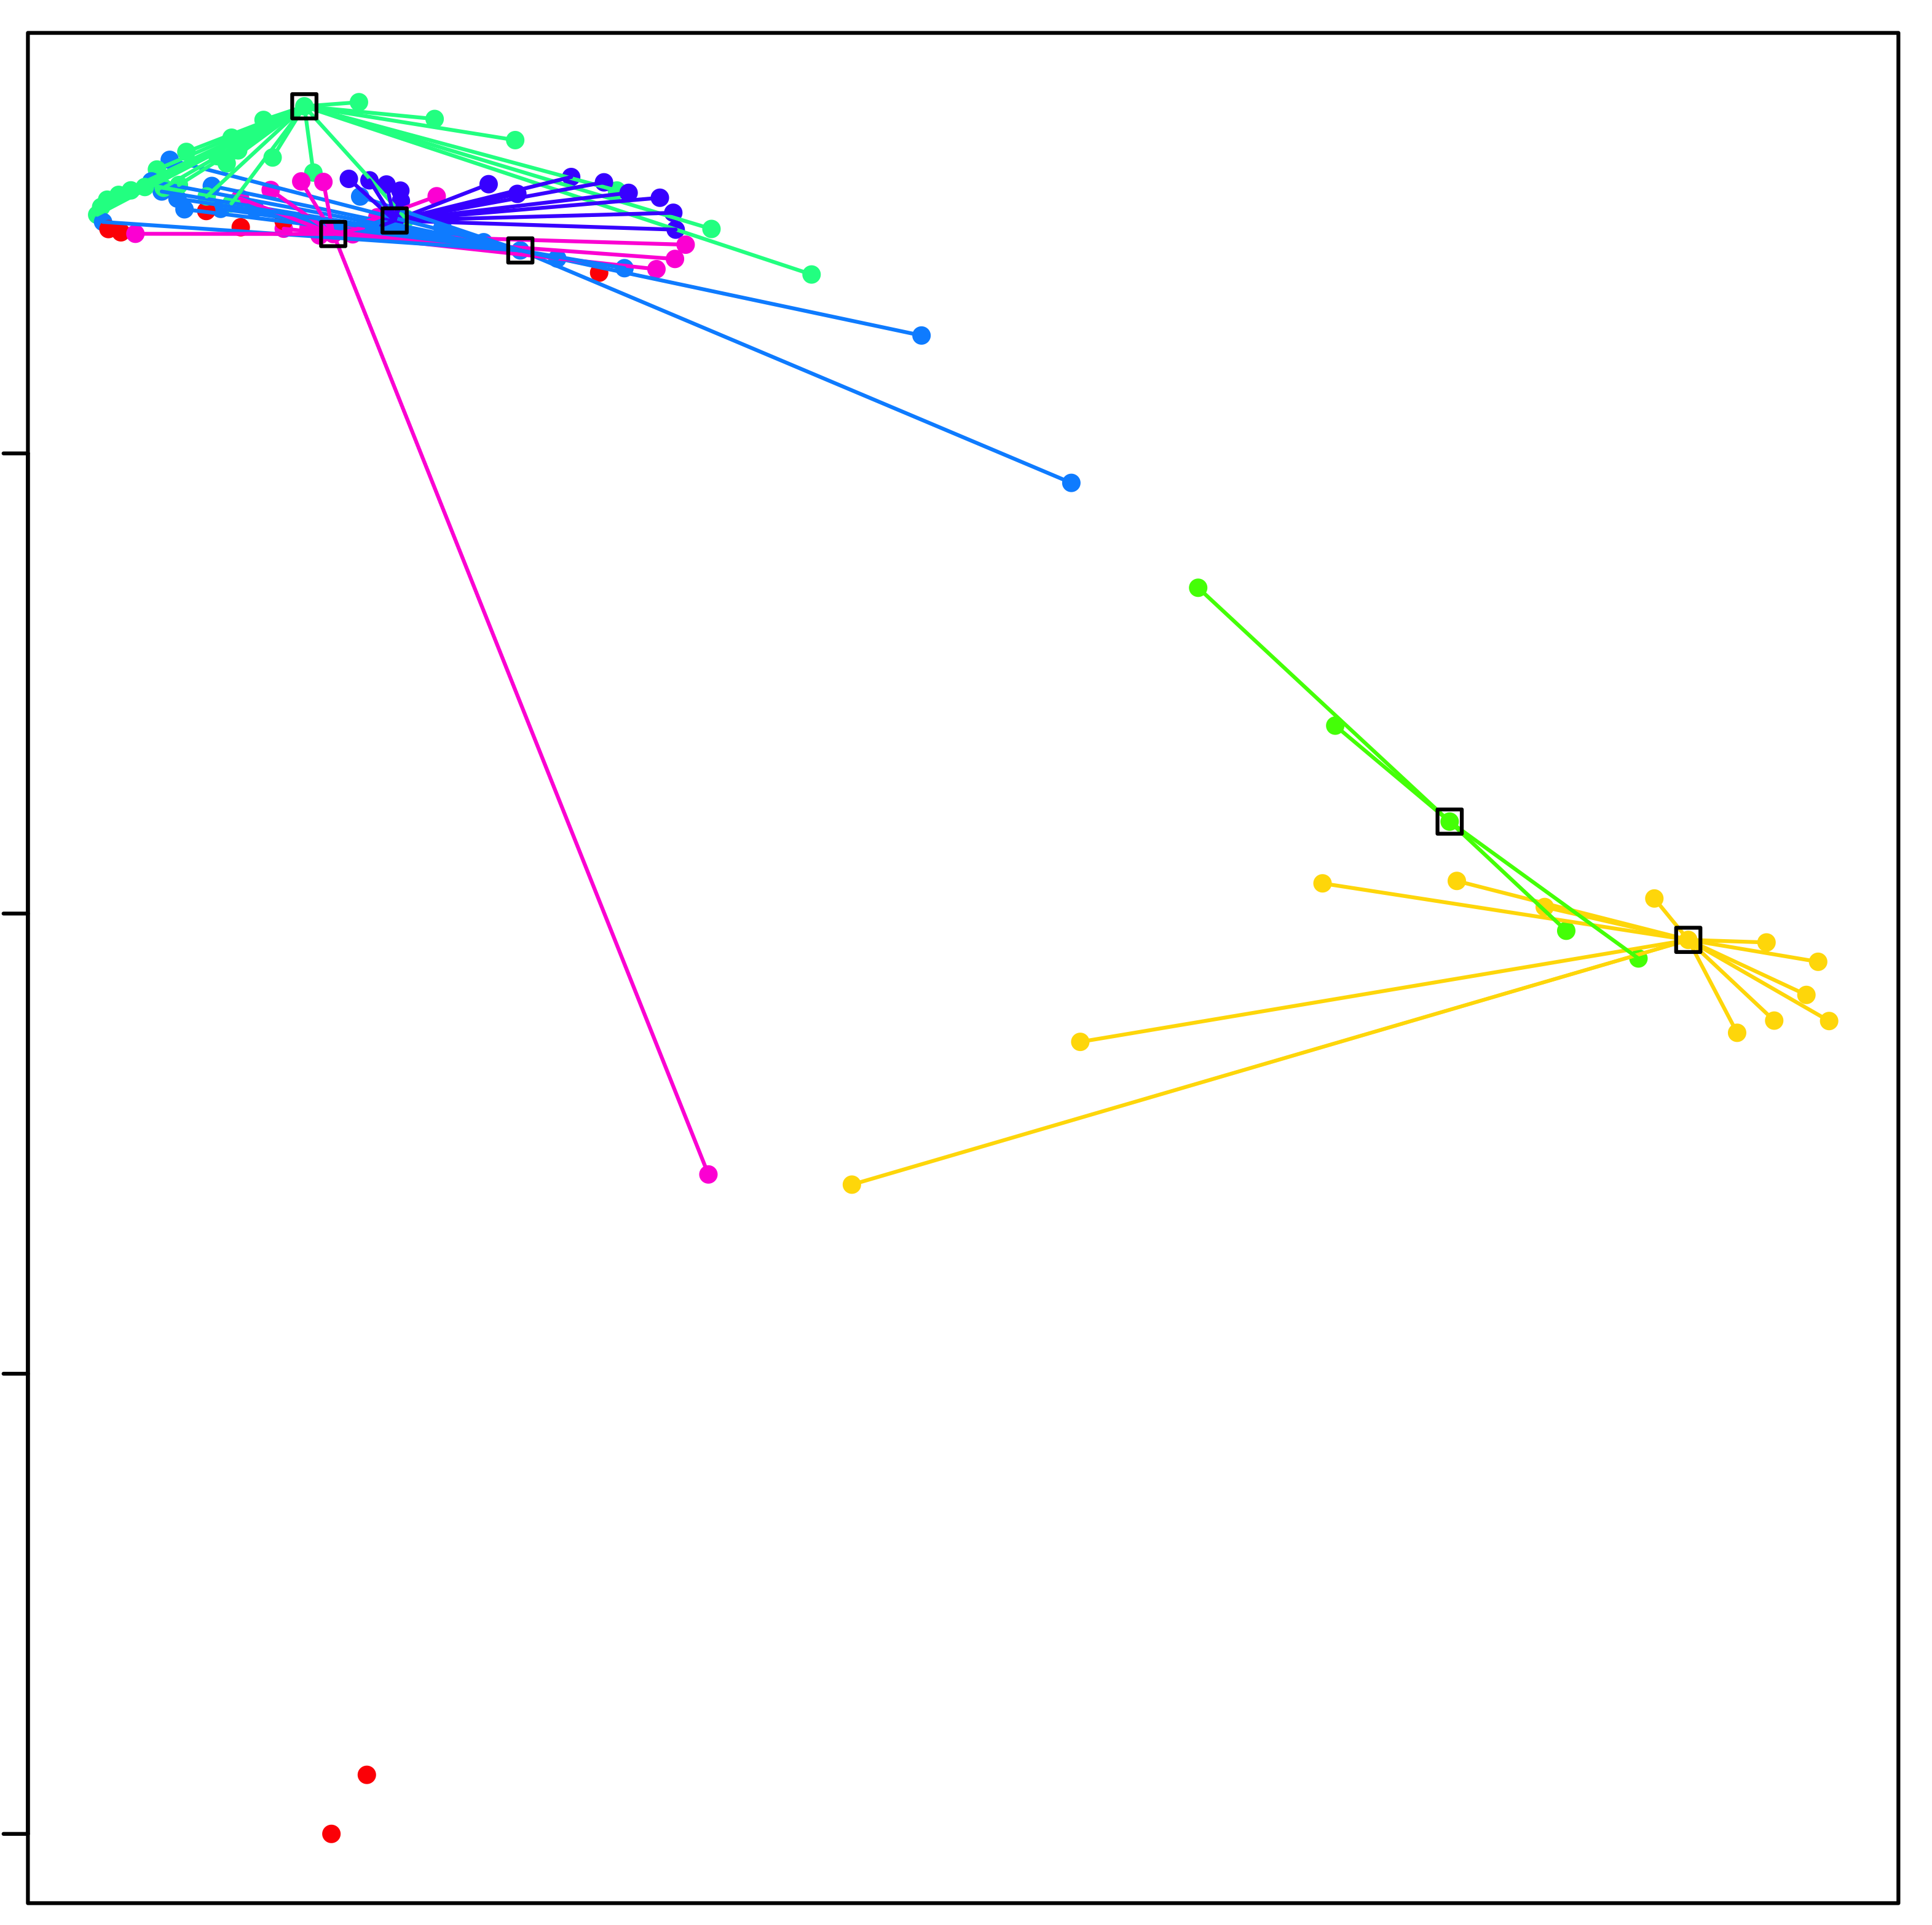
\includegraphics[height=\textwidth]{./gfx/ap12.png}
    \caption{Affinity Propagation clustering.\label{fig:avgstd:ap}}
  \end{subfigure}

  \caption{Average vs.\ Standard Deviation clustering.\label{fig:avgstd}}
\end{figure}

\begin{figure}[htbp]
  \centering
  \begin{subfigure}[b]{0.32\textwidth}
    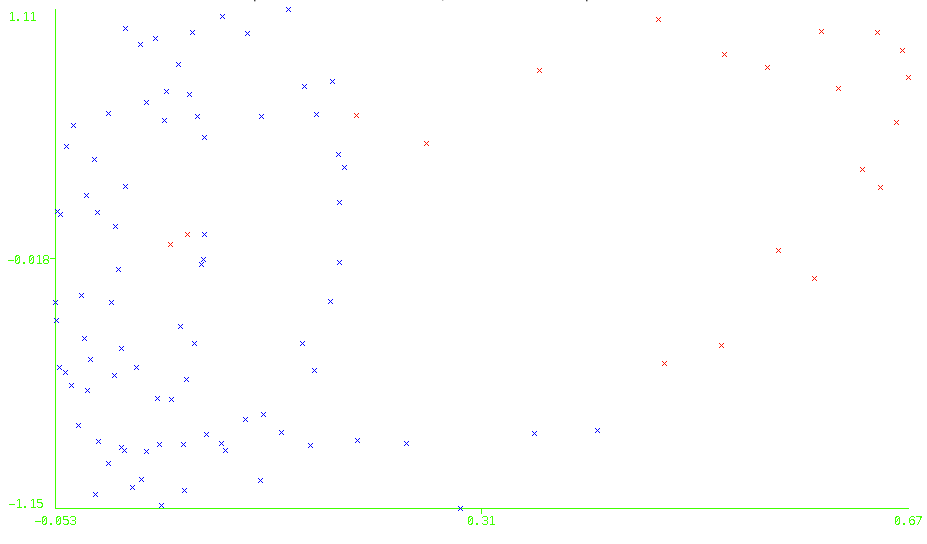
\includegraphics[width=\textwidth]{./gfx/km15.png}
    \caption{2-means clustering.\label{fig:svavg:km}}
  \end{subfigure}
  \hfill
  \begin{subfigure}[b]{0.32\textwidth}
    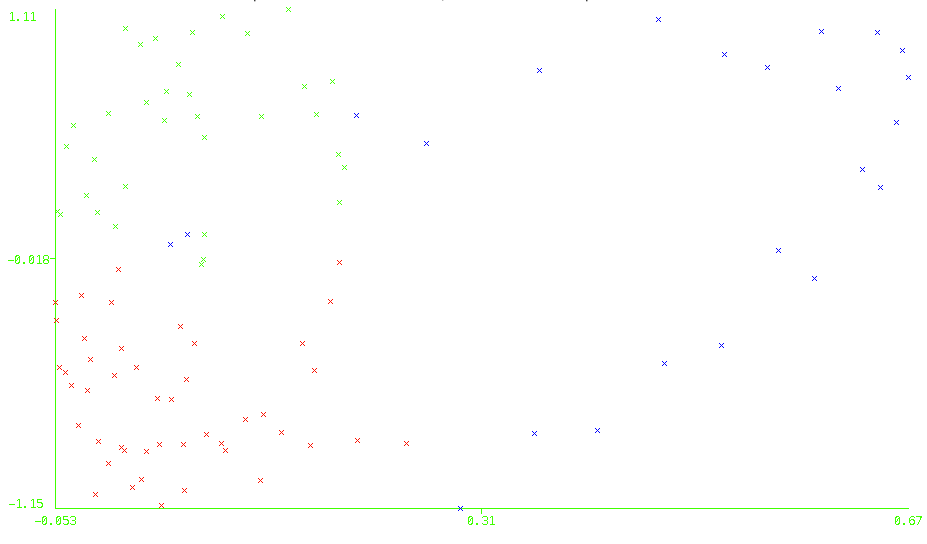
\includegraphics[width=\textwidth]{./gfx/em15.png}
    \caption{EM clustering.\label{fig:svavg:em}}
  \end{subfigure}
  \hfill
  \begin{subfigure}[b]{0.32\textwidth}
    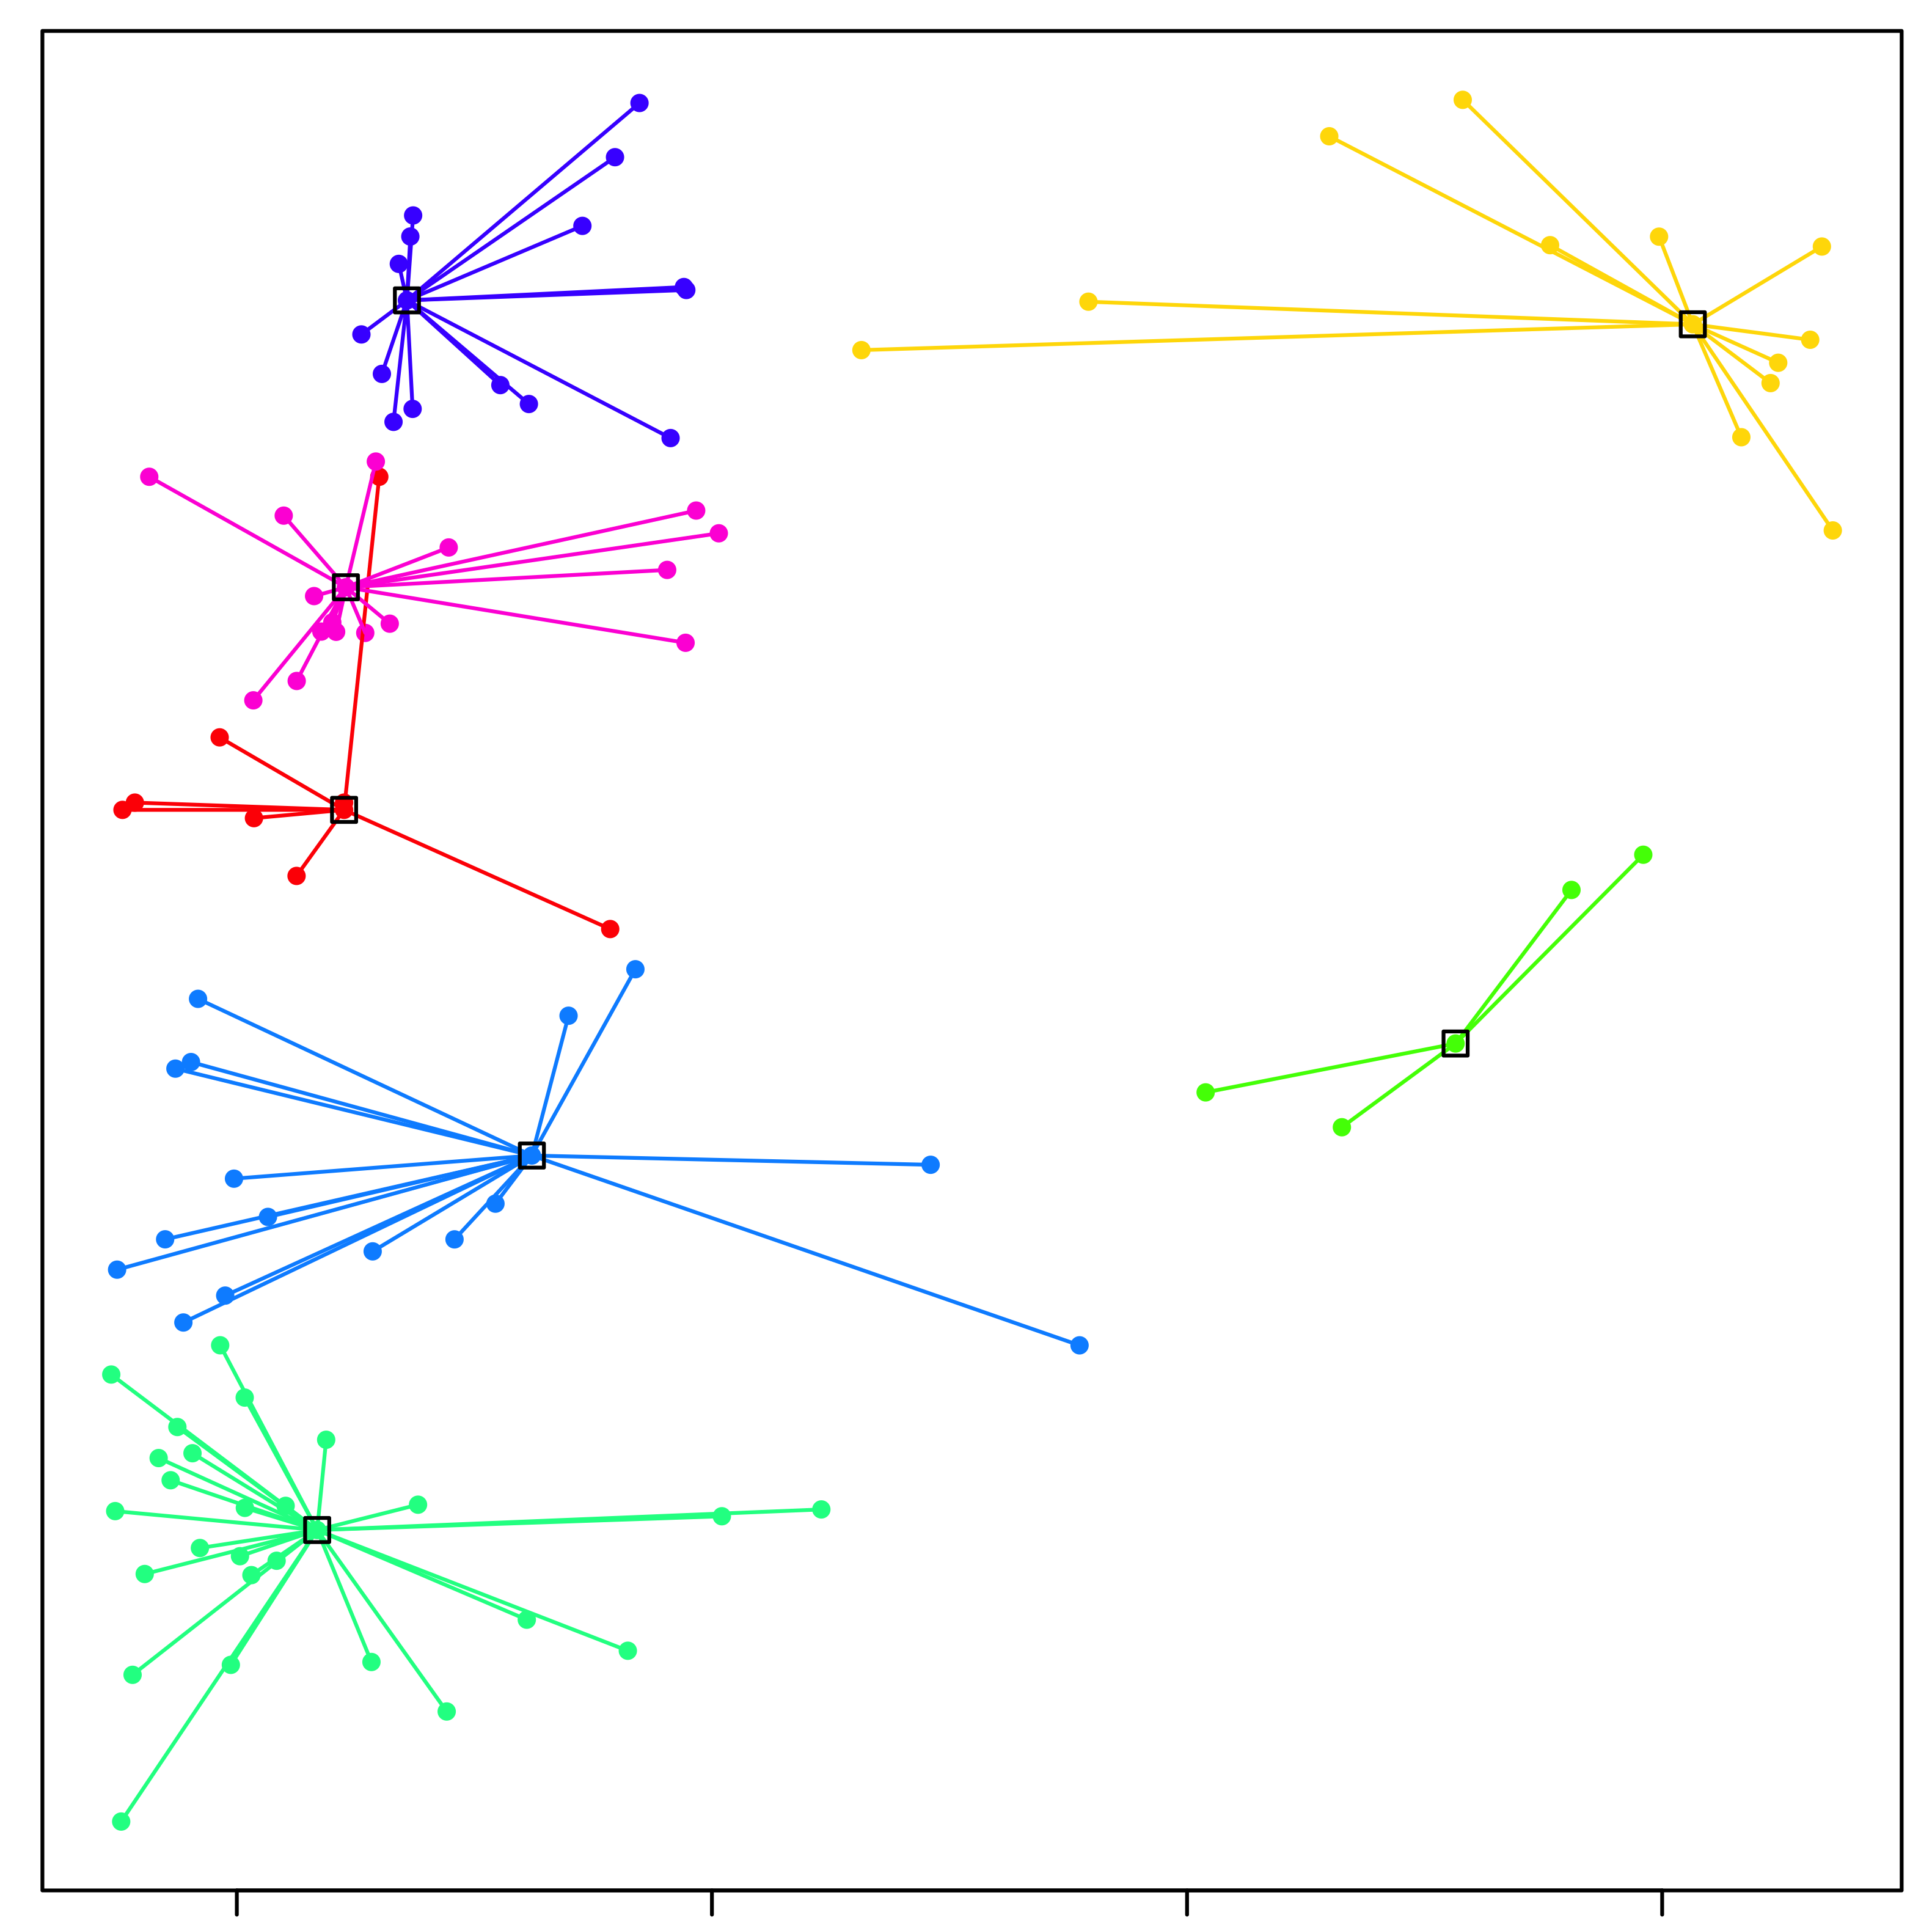
\includegraphics[height=\textwidth]{./gfx/ap15.png}
    \caption{Affinity Propagation clustering.\label{fig:svavg:ap}}
  \end{subfigure}

  \caption{Signal Value vs.\ Average clustering.\label{fig:svavg}}
\end{figure}

\begin{figure}[htbp]
  \centering
  \begin{subfigure}[b]{0.32\textwidth}
    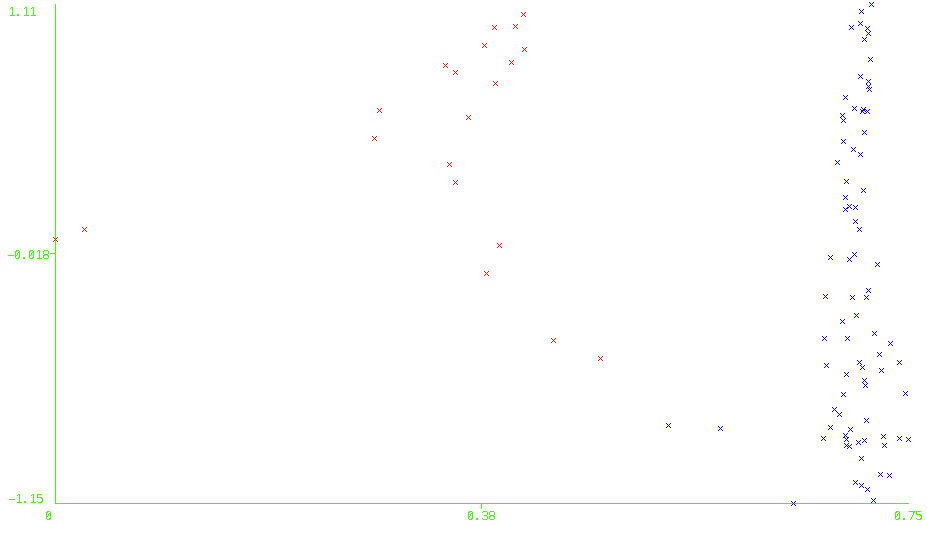
\includegraphics[width=\textwidth]{./gfx/km25.png}
    \caption{2-means clustering.\label{fig:svstd:km}}
  \end{subfigure}
  \hfill
  \begin{subfigure}[b]{0.32\textwidth}
    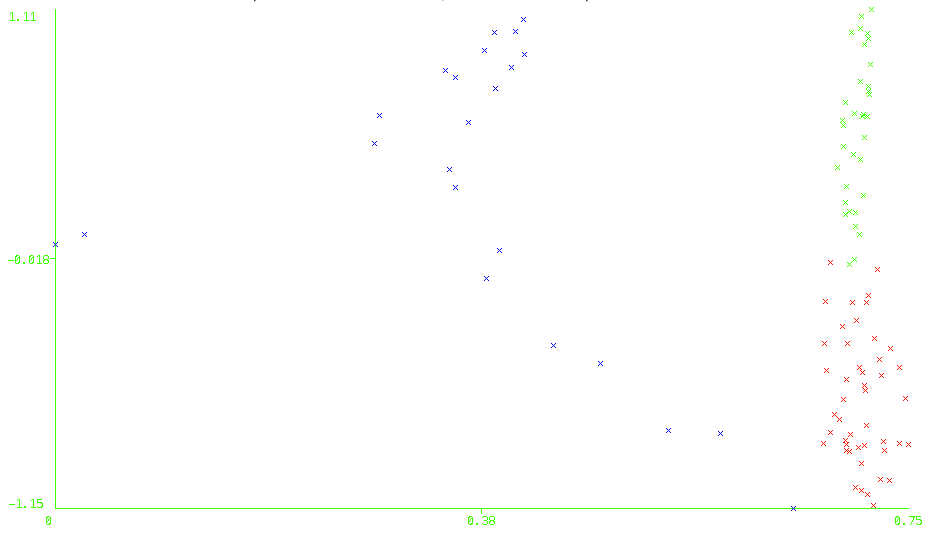
\includegraphics[width=\textwidth]{./gfx/em25.png}
    \caption{EM clustering.\label{fig:svstd:em}}
  \end{subfigure}
  \hfill
  \begin{subfigure}[b]{0.32\textwidth}
    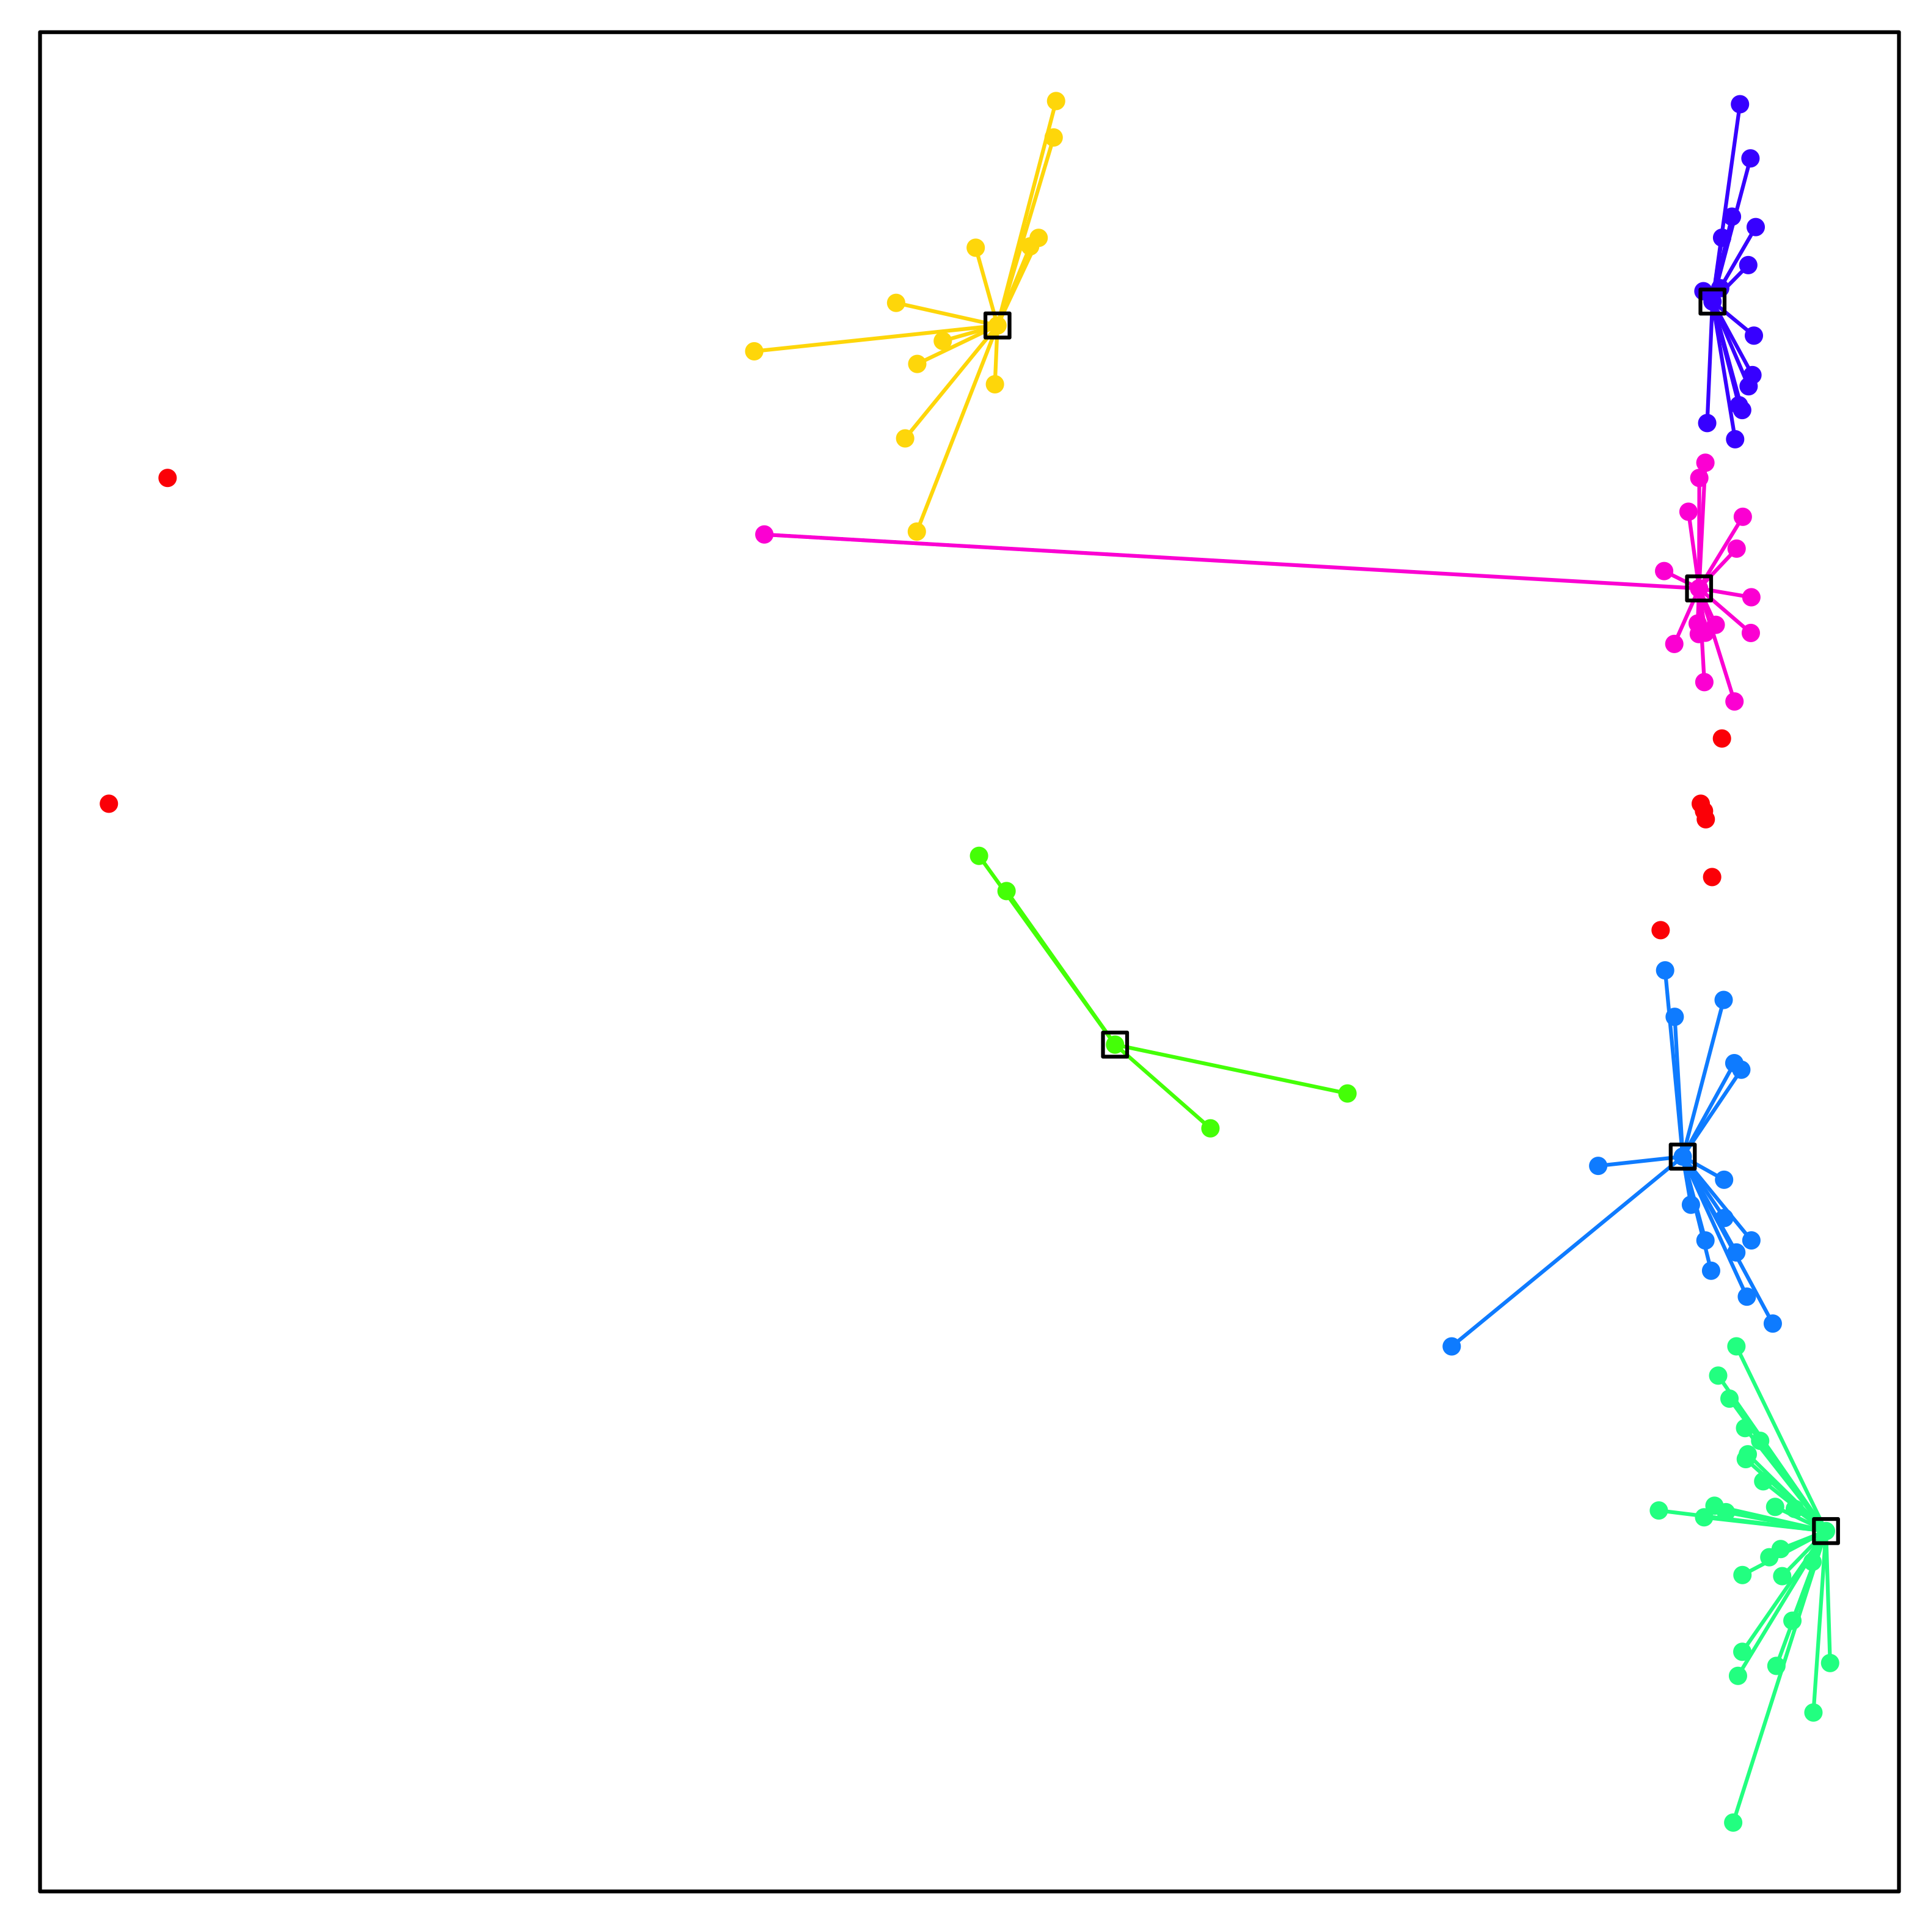
\includegraphics[height=\textwidth]{./gfx/ap25.png}
    \caption{Affinity Propagation clustering.\label{fig:svstd:ap}}
  \end{subfigure}

  \caption{Signal Value vs.\ Standard Deviation clustering.\label{fig:svstd}}
\end{figure}

\begin{figure}[htbp]
  \centering
  \begin{subfigure}[b]{0.32\textwidth}
    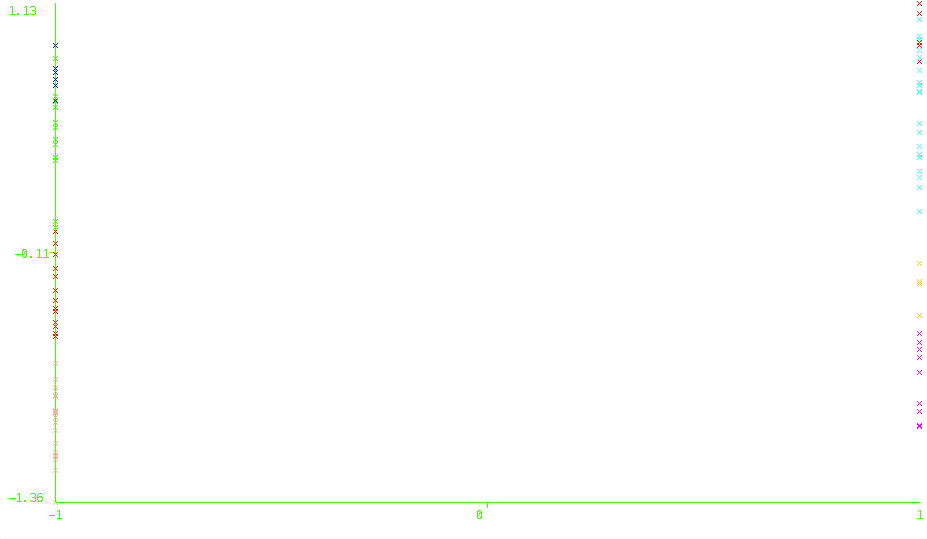
\includegraphics[width=\textwidth]{./gfx/km35.png}
    \caption{2-means clustering.\label{fig:svlag:km}}
  \end{subfigure}
  \hfill
  \begin{subfigure}[b]{0.32\textwidth}
    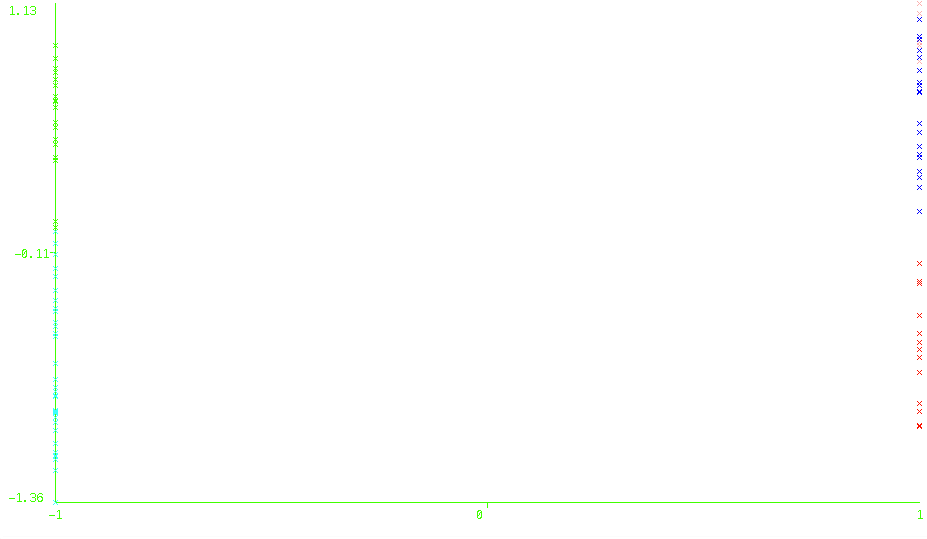
\includegraphics[width=\textwidth]{./gfx/em35.png}
    \caption{EM clustering.\label{fig:svlag:em}}
  \end{subfigure}
  \hfill
  \begin{subfigure}[b]{0.32\textwidth}
    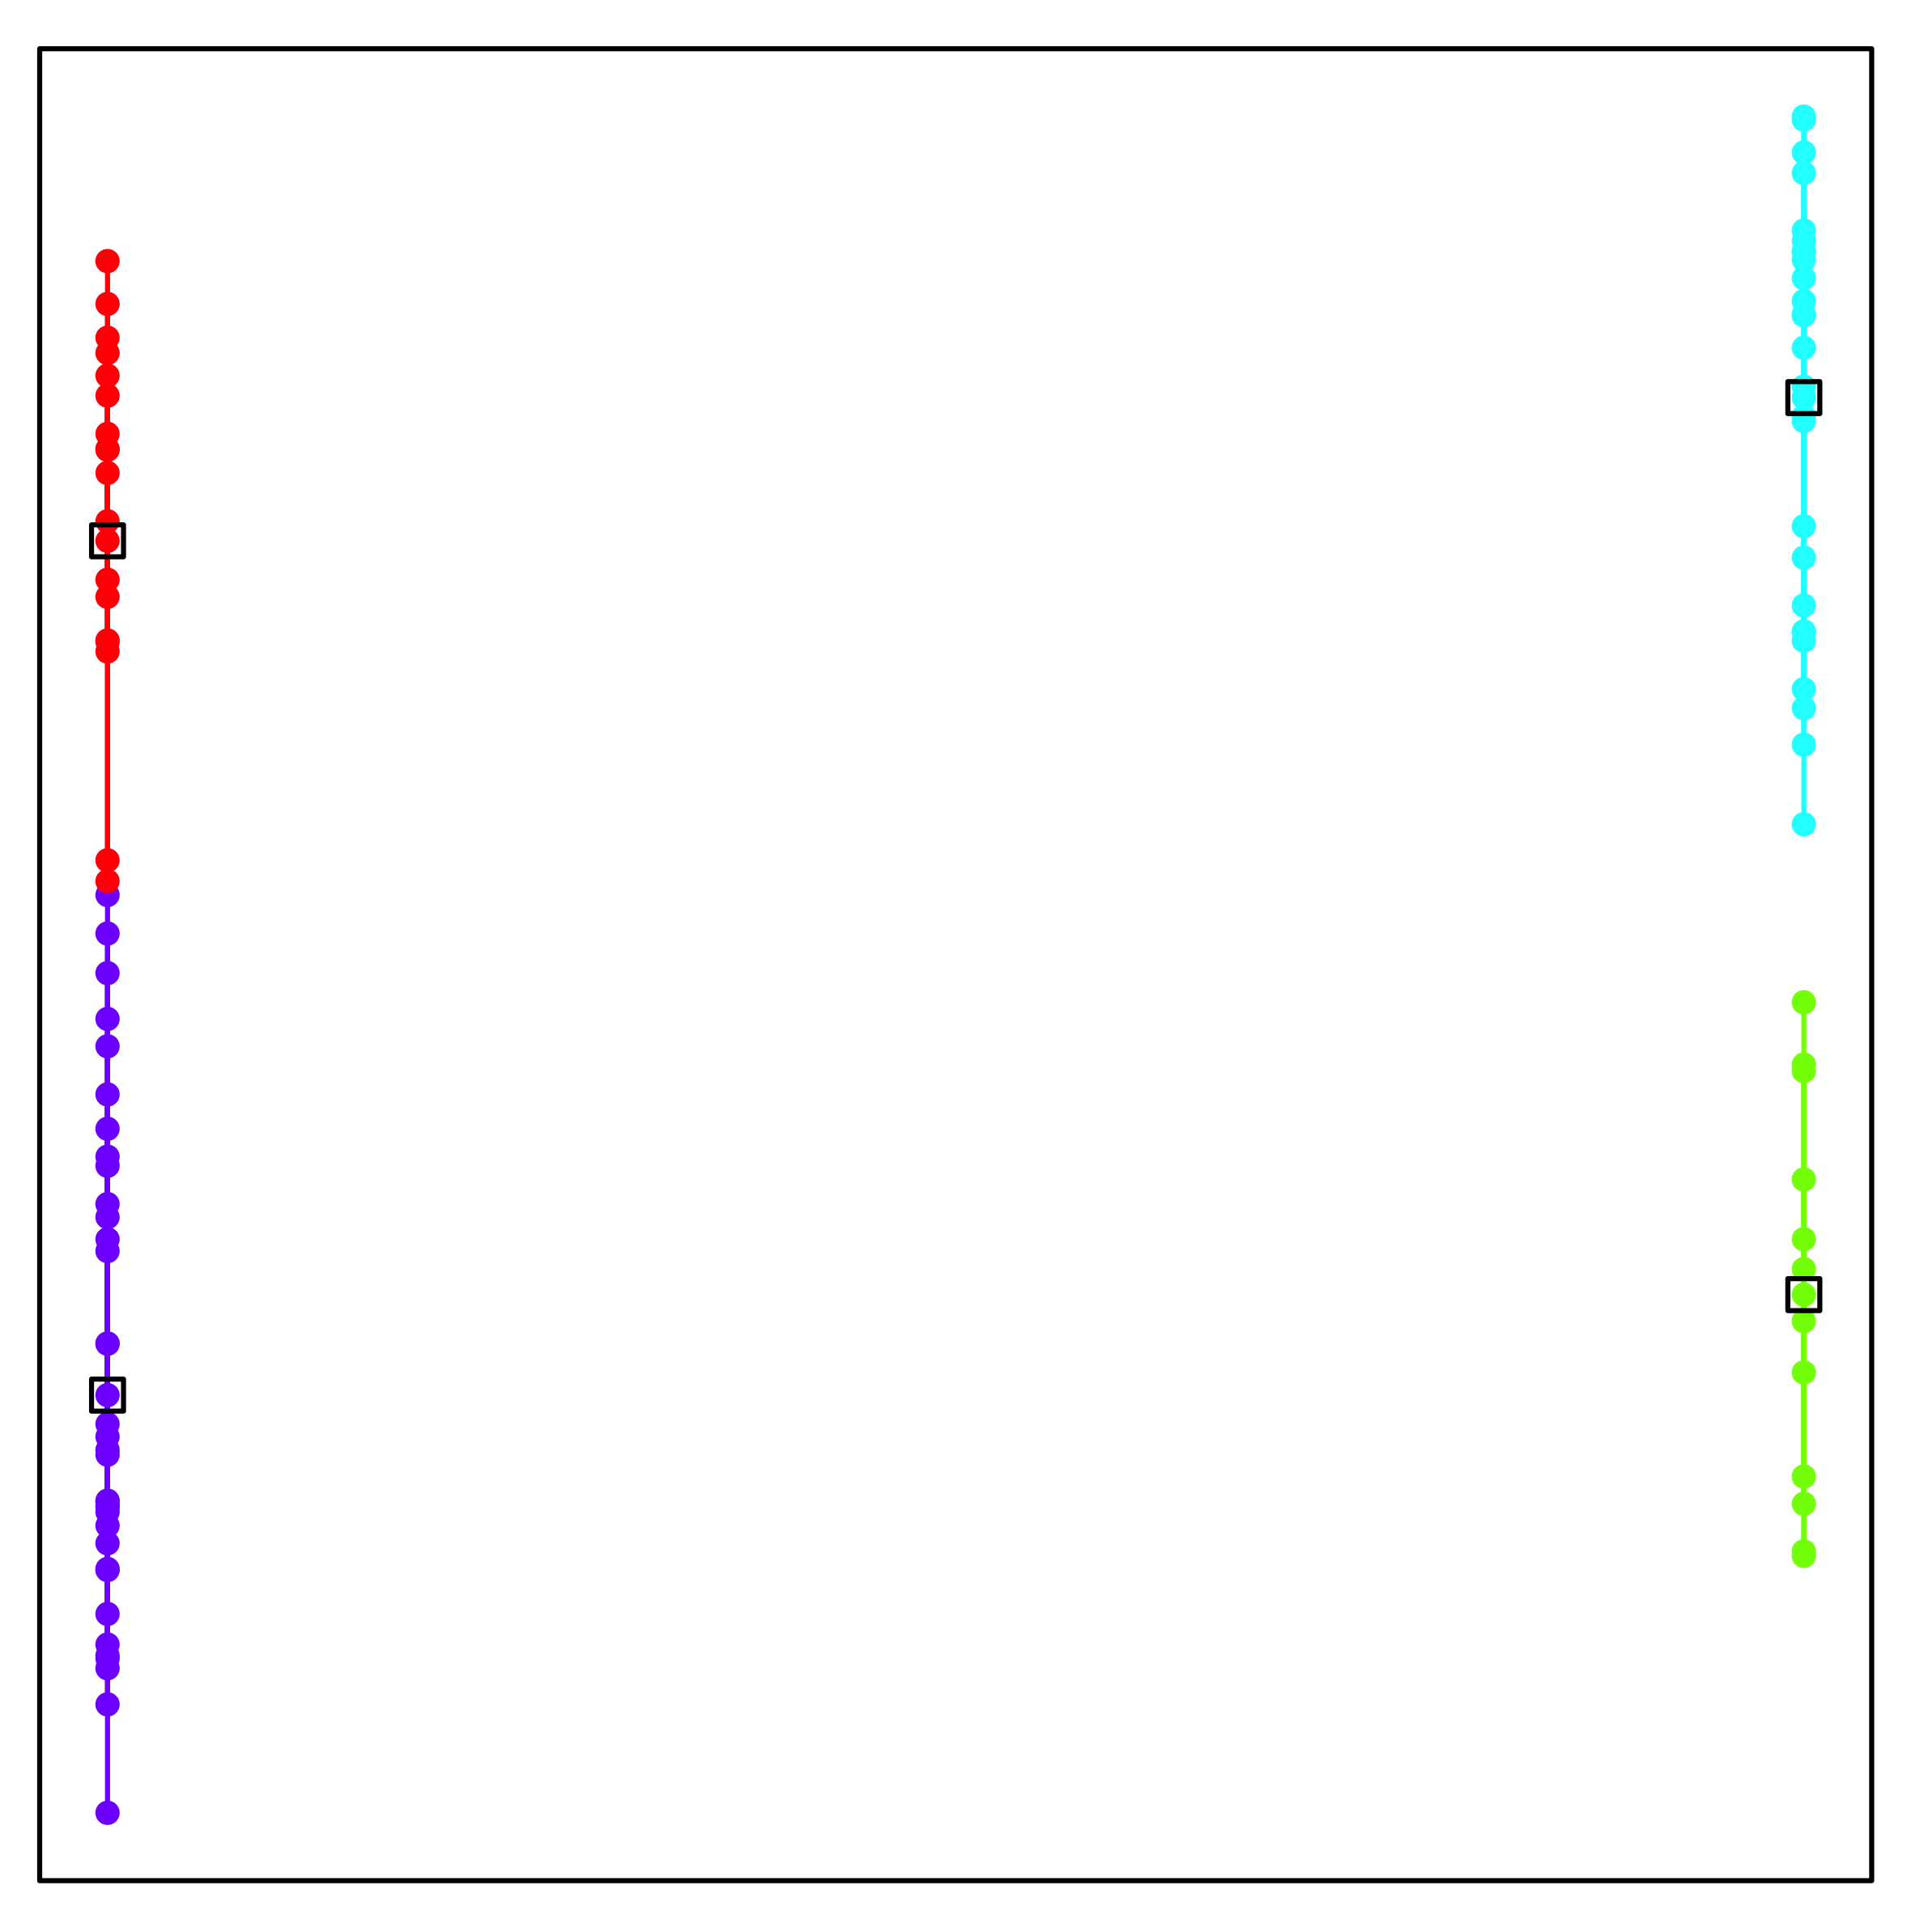
\includegraphics[height=\textwidth]{./gfx/ap35.png}
    \caption{Affinity Propagation clustering.\label{fig:svlag:ap}}
  \end{subfigure}

  \caption{Signal Value vs.\ 5-Lag clustering.\label{fig:svlag}}
\end{figure}

\section{Future work}
Created application only scratches the surface of a vast field of live signal analysis.\\
In further study I aim to address throughout comparison of different clustering algorithm that could be used with proposed framework. Another step worth taking is approach evaluation with real data.\\

The major lacking features of the application are: graphic interface which shows lively incoming signal, extracted features, and current cluster structure.\\
Furthermore, \texttt{Esper} facilitates new rules deployment on running application. Such possibility allows changing features of interest without stopping signal processing.\\

\section{Conclusions}
This paper proposes application of \emph{Complex Event Processing} tool \texttt{Esper} to \underline{make sense of data streams}. It covers all the processing steps from \emph{signal generation} through \emph{feature extraction} and \emph{data clustering}. Use of \texttt{Esper} brings all the advantages of efficient, multi-platform, and simple to us framework, which can process thousands of events produced by multiple signals per second.\\

Designed approach allows to analyze the live stream of data and automatically raise an alarm based on specified conditions. It can be used to monitor systems that demand more than simple signal thresholding.\\



\begin{center} \noindent \line(1,0){250} \end{center}       % Optional ending line


%% Start References (a.k.a. bibliography)
\newpage                                                                 % Optional new page before Bibliography
\bibliography{bibliography.bib}{}
\bibliographystyle{plainnat}

\end{document}
